% Options for packages loaded elsewhere
\PassOptionsToPackage{unicode}{hyperref}
\PassOptionsToPackage{hyphens}{url}
%
\documentclass[
  10pt,
  french,
  a5paper,
  openany]{book}
\usepackage{lmodern}
\usepackage{amssymb,amsmath}
\usepackage{ifxetex,ifluatex}
\ifnum 0\ifxetex 1\fi\ifluatex 1\fi=0 % if pdftex
  \usepackage[T1]{fontenc}
  \usepackage[utf8]{inputenc}
  \usepackage{textcomp} % provide euro and other symbols
\else % if luatex or xetex
  \usepackage{unicode-math}
  \defaultfontfeatures{Scale=MatchLowercase}
  \defaultfontfeatures[\rmfamily]{Ligatures=TeX,Scale=1}
\fi
% Use upquote if available, for straight quotes in verbatim environments
\IfFileExists{upquote.sty}{\usepackage{upquote}}{}
\IfFileExists{microtype.sty}{% use microtype if available
  \usepackage[]{microtype}
  \UseMicrotypeSet[protrusion]{basicmath} % disable protrusion for tt fonts
}{}
\makeatletter
\@ifundefined{KOMAClassName}{% if non-KOMA class
  \IfFileExists{parskip.sty}{%
    \usepackage{parskip}
  }{% else
    \setlength{\parindent}{0pt}
    \setlength{\parskip}{6pt plus 2pt minus 1pt}}
}{% if KOMA class
  \KOMAoptions{parskip=half}}
\makeatother
\usepackage{xcolor}
\IfFileExists{xurl.sty}{\usepackage{xurl}}{} % add URL line breaks if available
\IfFileExists{bookmark.sty}{\usepackage{bookmark}}{\usepackage{hyperref}}
\hypersetup{
  pdftitle={Travaux de maturité 2023},
  pdflang={fr},
  hidelinks,
  pdfcreator={LaTeX via pandoc}}
\urlstyle{same} % disable monospaced font for URLs
\usepackage[margin=20mm]{geometry}
\usepackage{longtable,booktabs}
% Correct order of tables after \paragraph or \subparagraph
\usepackage{etoolbox}
\makeatletter
\patchcmd\longtable{\par}{\if@noskipsec\mbox{}\fi\par}{}{}
\makeatother
% Allow footnotes in longtable head/foot
\IfFileExists{footnotehyper.sty}{\usepackage{footnotehyper}}{\usepackage{footnote}}
\makesavenoteenv{longtable}
\usepackage{graphicx,grffile}
\makeatletter
\def\maxwidth{\ifdim\Gin@nat@width>\linewidth\linewidth\else\Gin@nat@width\fi}
\def\maxheight{\ifdim\Gin@nat@height>\textheight\textheight\else\Gin@nat@height\fi}
\makeatother
% Scale images if necessary, so that they will not overflow the page
% margins by default, and it is still possible to overwrite the defaults
% using explicit options in \includegraphics[width, height, ...]{}
\setkeys{Gin}{width=\maxwidth,height=\maxheight,keepaspectratio}
% Set default figure placement to htbp
\makeatletter
\def\fps@figure{htbp}
\makeatother
\setlength{\emergencystretch}{3em} % prevent overfull lines
\providecommand{\tightlist}{%
  \setlength{\itemsep}{0pt}\setlength{\parskip}{0pt}}
\setcounter{secnumdepth}{5}
\usepackage[T1]{fontenc}
\usepackage[]{plex-otf}
\renewcommand*\familydefault{\sfdefault}

\widowpenalty10000
\clubpenalty10000

\renewcommand{\arraystretch}{1.5}

\setcounter{tocdepth}{1}

\usepackage{booktabs}
\usepackage{tabto}

\usepackage{fancyhdr}
\setlength{\headheight}{30pt}

\pagestyle{fancy}
\lhead{}
\chead{}
\rhead{\footnotesize Travaux de maturité 2023}
\lfoot{}
\cfoot{\footnotesize\thepage}
\rfoot{}
\renewcommand{\headrulewidth}{0.2pt}
\renewcommand{\footrulewidth}{0.2pt}

\fancypagestyle{plain}{
  \pagestyle{fancy}
  \lhead{}
  \chead{}
  \rhead{}
  \lfoot{}
  \cfoot{\footnotesize\thepage}
  \rfoot{}
  \renewcommand{\headrulewidth}{0pt}
  \renewcommand{\footrulewidth}{0.2pt}
}

\usepackage{titlesec}
\titlespacing{\chapter}{0em}{0em}{1em}
\titleformat{\chapter}[display]{\normalfont\bfseries\centering}{}{0pt}{\Large}
\titleformat{\section}[display]{\normalfont\bfseries}{}{0pt}{\large}
\titleformat{\subsection}[display]{\normalfont\bfseries}{}{0pt}{\normalsize}

\usepackage{tocbasic}
\DeclareTOCStyleEntry[
  indent=0pt,
  numwidth=0pt,
  raggedentrytext
]{tocline}{part}

\DeclareTOCStyleEntries[
  raggedentrytext
]{tocline}{chapter,section,subsection,subsubsection,paragraph,subparagraph}

\newenvironment{signature}{\begin{flushright}}{\end{flushright}}
\ifxetex
  % Load polyglossia as late as possible: uses bidi with RTL langages (e.g. Hebrew, Arabic)
  \usepackage{polyglossia}
  \setmainlanguage[]{french}
\else
  \usepackage[shorthands=off,main=french]{babel}
\fi

\title{Travaux de maturité 2023}
\author{}
\date{\vspace{-2.5em}05.11.2022}

\begin{document}
\maketitle

{
\setcounter{tocdepth}{0}
\tableofcontents
}
\hypertarget{lillustration-2023}{%
\chapter*{L'illustration 2023}\label{lillustration-2023}}
\addcontentsline{toc}{chapter}{L'illustration 2023}

L'illustration utilisée en couverture de l'édition de cette brochure est la photo gagnante d'un concours de macro-photographie organisé dans le cadre des laboraroires de chimie de la classe 2M21 pendant l'année scolaire 2021-2022.

Nos félicitations et nos remerciements vont aux auteurs de cette image : Élise Rollier et Yann Lopez (3M21).

\hypertarget{le-mot-du-doyen}{%
\chapter*{Le mot du doyen}\label{le-mot-du-doyen}}
\addcontentsline{toc}{chapter}{Le mot du doyen}


\includegraphics[width=\textwidth,height=5em]{images/logoGNLC.png}

\vspace{\stretch{1}}

\begin{signature}
\emph{À toutes et tous les élèves}\\
\emph{des classes de 2\textsuperscript{e} année}\\
\emph{de l'École de maturité}

\end{signature}

\vspace{\stretch{1}}

Chères élèves, chers élèves,

Vous recevez cette brochure qui concerne le travail de maturité pour la volée 2022-2023 et qui contient, en particulier, les thèmes des projets qui vous sont proposés.

Je vous donne rendez-vous le

\begin{center}
\textbf{Mardi 22 novembre à 11h05 ;\\
Espace Assemblée (en prolongement de la cafétéria)}

\end{center}

afin d'y recevoir une information générale sur l'organisation du travail de maturité.

Vous aurez ensuite la possibilité de suivre la présentation de trois projets que vous aurez retenus parmi les pages qui suivent. Les présentations se dérouleront comme suit :

\begin{itemize}
\tightlist
\item
  la première de 11h55 à 12h20,
\item
  la seconde de 12h25 à 12h50 et
\item
  la troisième de 12h55 à 13h30.
\end{itemize}

Les cours seront donc interrompus ce jour de 10h50 à 13h30 pour les classes de 2M. Ils reprendront à 13h35 selon l'horaire habituel.

\clearpage

Après ces présentations, vous aurez à choisir trois thèmes. Vous devrez vous inscrire via le site du Gymnase de Nyon (\url{www.gymnasedenyon.ch}) en cliquant dans le menu

\begin{center}
``Intranet \textgreater{} Elèves \textgreater{} Horaires et Inscriptions'' puis ``Inscriptions''

\end{center}

et en respectant le délai fixé au \textbf{mercredi 30 novembre à 16h00}. Vous devrez formuler 3 souhaits, dans l'ordre de préférence. Les inscriptions définitives vous seront confirmées ultérieurement.

Avec mes meilleures salutations,

\begin{signature}
Le doyen\\
M. Rizzello

\end{signature}

\vspace{\stretch{1}}

Distribution à :

\begin{itemize}
\tightlist
\item
  toutes les classes de 2M
\item
  Conseil de direction
\item
  Mmes et MM. les maître·sse·s de classe de 2M
\item
  Mmes et MM. les responsables de projets, avec prière d'assister à cette séance d'information et de présenter les propositions de projets dans les salles qui seront attribuées
\end{itemize}

\hypertarget{attribution-des-salles}{%
\chapter*{Attribution des salles}\label{attribution-des-salles}}
\addcontentsline{toc}{chapter}{Attribution des salles}

\begin{longtable}[]{@{}lc@{}}
\toprule
\begin{minipage}[b]{0.88\columnwidth}\raggedright
Thème\strut
\end{minipage} & \begin{minipage}[b]{0.06\columnwidth}\centering
Salle n°\strut
\end{minipage}\tabularnewline
\midrule
\endhead
\begin{minipage}[t]{0.88\columnwidth}\raggedright
Le conte écrit transposé au cinéma\strut
\end{minipage} & \begin{minipage}[t]{0.06\columnwidth}\centering
\textasciitilde{}\strut
\end{minipage}\tabularnewline
\begin{minipage}[t]{0.88\columnwidth}\raggedright
Réécriture de contes\strut
\end{minipage} & \begin{minipage}[t]{0.06\columnwidth}\centering
\textasciitilde{}\strut
\end{minipage}\tabularnewline
\begin{minipage}[t]{0.88\columnwidth}\raggedright
Un conte et des conteurs\strut
\end{minipage} & \begin{minipage}[t]{0.06\columnwidth}\centering
\textasciitilde{}\strut
\end{minipage}\tabularnewline
\begin{minipage}[t]{0.88\columnwidth}\raggedright
Journaux (littérature personnelle)\strut
\end{minipage} & \begin{minipage}[t]{0.06\columnwidth}\centering
\textasciitilde{}\strut
\end{minipage}\tabularnewline
\begin{minipage}[t]{0.88\columnwidth}\raggedright
Les machines et la communication : outils et sensibilités\strut
\end{minipage} & \begin{minipage}[t]{0.06\columnwidth}\centering
\textasciitilde{}\strut
\end{minipage}\tabularnewline
\begin{minipage}[t]{0.88\columnwidth}\raggedright
Représentations des figures héroïques (ou non) dans les bandes dessinées (DC, Marvel, mangas \ldots)\strut
\end{minipage} & \begin{minipage}[t]{0.06\columnwidth}\centering
\textasciitilde{}\strut
\end{minipage}\tabularnewline
\begin{minipage}[t]{0.88\columnwidth}\raggedright
Élaboration d'un guide de voyage dans une ville germanophone\strut
\end{minipage} & \begin{minipage}[t]{0.06\columnwidth}\centering
\textasciitilde{}\strut
\end{minipage}\tabularnewline
\begin{minipage}[t]{0.88\columnwidth}\raggedright
Le récit de voyage\strut
\end{minipage} & \begin{minipage}[t]{0.06\columnwidth}\centering
\textasciitilde{}\strut
\end{minipage}\tabularnewline
\begin{minipage}[t]{0.88\columnwidth}\raggedright
Multiculturalité et langage\strut
\end{minipage} & \begin{minipage}[t]{0.06\columnwidth}\centering
\textasciitilde{}\strut
\end{minipage}\tabularnewline
\begin{minipage}[t]{0.88\columnwidth}\raggedright
Les nombres remarquables\strut
\end{minipage} & \begin{minipage}[t]{0.06\columnwidth}\centering
\textasciitilde{}\strut
\end{minipage}\tabularnewline
\begin{minipage}[t]{0.88\columnwidth}\raggedright
La géométrie non euclidienne\strut
\end{minipage} & \begin{minipage}[t]{0.06\columnwidth}\centering
\textasciitilde{}\strut
\end{minipage}\tabularnewline
\begin{minipage}[t]{0.88\columnwidth}\raggedright
Les défis de l'alimentation\strut
\end{minipage} & \begin{minipage}[t]{0.06\columnwidth}\centering
\textasciitilde{}\strut
\end{minipage}\tabularnewline
\begin{minipage}[t]{0.88\columnwidth}\raggedright
Étude de la biodiversité\strut
\end{minipage} & \begin{minipage}[t]{0.06\columnwidth}\centering
\textasciitilde{}\strut
\end{minipage}\tabularnewline
\begin{minipage}[t]{0.88\columnwidth}\raggedright
L'intelligence artificielle est-elle vraiment intelligente ?\strut
\end{minipage} & \begin{minipage}[t]{0.06\columnwidth}\centering
\textasciitilde{}\strut
\end{minipage}\tabularnewline
\begin{minipage}[t]{0.88\columnwidth}\raggedright
Santé et sport\strut
\end{minipage} & \begin{minipage}[t]{0.06\columnwidth}\centering
\textasciitilde{}\strut
\end{minipage}\tabularnewline
\begin{minipage}[t]{0.88\columnwidth}\raggedright
Le sommeil\strut
\end{minipage} & \begin{minipage}[t]{0.06\columnwidth}\centering
\textasciitilde{}\strut
\end{minipage}\tabularnewline
\begin{minipage}[t]{0.88\columnwidth}\raggedright
Des analyses chimiques avec mon téléphone portable\strut
\end{minipage} & \begin{minipage}[t]{0.06\columnwidth}\centering
\textasciitilde{}\strut
\end{minipage}\tabularnewline
\begin{minipage}[t]{0.88\columnwidth}\raggedright
Chimie et photographie\strut
\end{minipage} & \begin{minipage}[t]{0.06\columnwidth}\centering
\textasciitilde{}\strut
\end{minipage}\tabularnewline
\begin{minipage}[t]{0.88\columnwidth}\raggedright
L'eau chaude gèle-t-elle plus vite que l'eau froide ?\strut
\end{minipage} & \begin{minipage}[t]{0.06\columnwidth}\centering
\textasciitilde{}\strut
\end{minipage}\tabularnewline
\begin{minipage}[t]{0.88\columnwidth}\raggedright
Les additifs en cosmétiques\strut
\end{minipage} & \begin{minipage}[t]{0.06\columnwidth}\centering
\textasciitilde{}\strut
\end{minipage}\tabularnewline
\begin{minipage}[t]{0.88\columnwidth}\raggedright
Fluorescence et phosphorescence\strut
\end{minipage} & \begin{minipage}[t]{0.06\columnwidth}\centering
\textasciitilde{}\strut
\end{minipage}\tabularnewline
\begin{minipage}[t]{0.88\columnwidth}\raggedright
C'est pas sorcier\strut
\end{minipage} & \begin{minipage}[t]{0.06\columnwidth}\centering
\textasciitilde{}\strut
\end{minipage}\tabularnewline
\begin{minipage}[t]{0.88\columnwidth}\raggedright
Changement climatique et sociétés\strut
\end{minipage} & \begin{minipage}[t]{0.06\columnwidth}\centering
\textasciitilde{}\strut
\end{minipage}\tabularnewline
\begin{minipage}[t]{0.88\columnwidth}\raggedright
L'équilibre entre la vie professionnelle et la vie privé des jeunes adultes\strut
\end{minipage} & \begin{minipage}[t]{0.06\columnwidth}\centering
\textasciitilde{}\strut
\end{minipage}\tabularnewline
\begin{minipage}[t]{0.88\columnwidth}\raggedright
Le droit dans l'univers d'Harry Potter\strut
\end{minipage} & \begin{minipage}[t]{0.06\columnwidth}\centering
\textasciitilde{}\strut
\end{minipage}\tabularnewline
\begin{minipage}[t]{0.88\columnwidth}\raggedright
Philosophie de l'art : La beauté et la vérité\strut
\end{minipage} & \begin{minipage}[t]{0.06\columnwidth}\centering
\textasciitilde{}\strut
\end{minipage}\tabularnewline
\begin{minipage}[t]{0.88\columnwidth}\raggedright
Au-delà de l'humain : transhumanisme et intelligence artificielle, quelles représentations et quels enjeux ?\strut
\end{minipage} & \begin{minipage}[t]{0.06\columnwidth}\centering
\textasciitilde{}\strut
\end{minipage}\tabularnewline
\begin{minipage}[t]{0.88\columnwidth}\raggedright
Le jeu vidéo : fiction ou réalité ?\strut
\end{minipage} & \begin{minipage}[t]{0.06\columnwidth}\centering
\textasciitilde{}\strut
\end{minipage}\tabularnewline
\begin{minipage}[t]{0.88\columnwidth}\raggedright
Ecritures d'artistes, histoire d'écritures : évolutions et appropriations de l'écriture\strut
\end{minipage} & \begin{minipage}[t]{0.06\columnwidth}\centering
\textasciitilde{}\strut
\end{minipage}\tabularnewline
\begin{minipage}[t]{0.88\columnwidth}\raggedright
Composition et Réalisation d'un EP / clip vidéo musical\strut
\end{minipage} & \begin{minipage}[t]{0.06\columnwidth}\centering
\textasciitilde{}\strut
\end{minipage}\tabularnewline
\begin{minipage}[t]{0.88\columnwidth}\raggedright
Organisation d'un concert public\strut
\end{minipage} & \begin{minipage}[t]{0.06\columnwidth}\centering
\textasciitilde{}\strut
\end{minipage}\tabularnewline
\bottomrule
\end{longtable}

\hypertarget{rappel-des-dispositions-ruxe8glementaires}{%
\chapter*{Rappel des dispositions règlementaires}\label{rappel-des-dispositions-ruxe8glementaires}}
\addcontentsline{toc}{chapter}{Rappel des dispositions règlementaires}

\hypertarget{ruxe8glement-du-16-janvier-1995-sur-la-reconnaissance-des-certificats-de-maturituxe9-gymnasiale-rrm}{%
\subsection*{Règlement du 16 janvier 1995 sur la reconnaissance des certificats de maturité gymnasiale (RRM)}\label{ruxe8glement-du-16-janvier-1995-sur-la-reconnaissance-des-certificats-de-maturituxe9-gymnasiale-rrm}}
\addcontentsline{toc}{subsection}{Règlement du 16 janvier 1995 sur la reconnaissance des certificats de maturité gymnasiale (RRM)}

\emph{{[}édicté par la Conférence suisse des Directeurs cantonaux de l'instruction publique (CDIP) ; état au 1er août 2007{]}}

\vspace{\stretch{1}}

\emph{Art. 9 Disciplines de maturité}

\begin{enumerate}
\def\labelenumi{\arabic{enumi}.}
\tightlist
\item
  Les disciplines fondamentales, l'option spécifique, l'option complémentaire et le travail de maturité constituent l'ensemble des disciplines de la maturité.
\end{enumerate}

(\ldots)

\vspace{\stretch{1}}

\emph{Art. 10 Travail de maturité}

Chaque élève doit effectuer, seul ou en équipe, un travail autonome d'une certaine importance. Ce travail fera l'objet d'un texte ou d'un commentaire rédigé et d'une présentation orale.

\vspace{\stretch{1}}

\emph{Art.15 Notes de maturité et évaluation du travail de maturité}

(\ldots)

\begin{enumerate}
\def\labelenumi{\arabic{enumi}.}
\setcounter{enumi}{1}
\tightlist
\item
  Le travail de maturité est évalué sur la base des prestations écrites et orales.
\end{enumerate}

\vspace{\stretch{1}}

\clearpage

\hypertarget{ruxe8glement-des-gymnases-du-6-juillet-2016-rgy}{%
\subsection*{Règlement des gymnases du 6 juillet 2016 (RGY)}\label{ruxe8glement-des-gymnases-du-6-juillet-2016-rgy}}
\addcontentsline{toc}{subsection}{Règlement des gymnases du 6 juillet 2016 (RGY)}

\emph{{[}édicté par le Conseil d'État du Canton de Vaud{]}}

\emph{Art.82 Travail de maturité}

\begin{enumerate}
\def\labelenumi{\arabic{enumi}.}
\tightlist
\item
  Les élèves effectuent un travail de maturité, seuls ou en équipe, entre la 2ème etla 3ème années, selon le calendrier fixé par le directeur et les modalités fixées par le département.
\item
  Le travail de maturité est évalué par un jury interne qui peut, le cas échéant, s'adjoindre un expert externe, sur la base de la mise en œuvre du projet, du document écrit déposé et de la présentation orale.
\item
  Le travail de maturité donne lieu à une note annuelle en 3ème année.
\item
  Le titre du travail de maturité est mentionné sur le certificat de maturité gymnasiale.
\item
  L'élève qui répète la 3ème année choisit, pour le début de l'année scolaire, soit de conserver sa note, soit d'effectuer un nouveau travail de maturité. Dans ce dernier cas, la note attribuée au premier travail n'est pas conservée.
\end{enumerate}

(\ldots)

\hypertarget{objectifs-et-uxe9valuation}{%
\chapter*{Objectifs et évaluation}\label{objectifs-et-uxe9valuation}}
\addcontentsline{toc}{chapter}{Objectifs et évaluation}

\hypertarget{principes-fondamentaux}{%
\section*{Principes fondamentaux}\label{principes-fondamentaux}}
\addcontentsline{toc}{section}{Principes fondamentaux}

Le travail de maturité est l'occasion pour l'élève, à l'issue d'un processus de longue durée, de parvenir à une assise, une ``maturité'' intellectuelle suffisamment solide pour pouvoir produire un discours ou une œuvre qu'il peut assumer en tant qu'auteur et soumettre au regard d'autrui. En d'autres termes, il s'agit pour lui de se constituer comme sujet d'une énonciation.

\hypertarget{objectifs-fondamentaux}{%
\section*{Objectifs fondamentaux}\label{objectifs-fondamentaux}}
\addcontentsline{toc}{section}{Objectifs fondamentaux}

Fondamentalement, il doit, pour parvenir à cela, être capable de :

\begin{itemize}
\tightlist
\item
  mener une recherche documentaire de qualité ;
\item
  structurer sa pensée, afin de progresser vers un but, qui consiste à résoudre un problème ;
\item
  formuler sa pensée pour la rendre intelligible à autrui ;
\item
  évaluer sa propre démarche et distinguer clairement sa position personnelle d'autres points de vue, en justifiant ses choix.
\end{itemize}

\hypertarget{uxe9valuation}{%
\section*{Évaluation}\label{uxe9valuation}}
\addcontentsline{toc}{section}{Évaluation}

\hypertarget{relation-puxe9dagogique}{%
\subsection*{Relation pédagogique}\label{relation-puxe9dagogique}}
\addcontentsline{toc}{subsection}{Relation pédagogique}

Le travail de maturité s'élabore sous la conduite d'un maître répondant. Il s'agit d'un processus de longue durée, qui doit être considéré comme une situation d'enseignement, ce qui implique un suivi et des échanges réguliers entre le répondant et l'élève.

En entreprenant son travail de maturité, l'élève s'engage dans une relation de collaboration avec son répondant : cela suppose que le contact soit cultivé de part et d'autre.

\hypertarget{uxe9valuation-1}{%
\subsection*{Évaluation}\label{uxe9valuation-1}}
\addcontentsline{toc}{subsection}{Évaluation}

L'évaluation du travail de maturité (travail d'analyse ou de création) porte sur les six domaines de compétence suivants :

\begin{itemize}
\tightlist
\item
  Recherche et méthodes de travail
\item
  Contenu et sens
\item
  Structure de l'opuscule
\item
  Sens critique, lucidité sur son travail
\item
  Expression
\item
  Présentation
\end{itemize}

\hypertarget{calendrier-pour-la-voluxe9e-2023}{%
\chapter*{Calendrier pour la volée 2023}\label{calendrier-pour-la-voluxe9e-2023}}
\addcontentsline{toc}{chapter}{Calendrier pour la volée 2023}

\vspace{\stretch{1}}

\textbf{1. Phase préparatoire \hfill septembre - décembre 2022}

\begin{longtable}[]{@{}ll@{}}
\toprule
\endhead
Propositions de projets &\tabularnewline
Constitution des équipes de projets &\tabularnewline
Information générale aux élèves de 2M &\tabularnewline
Présentation des projets par les équipes de maîtres &\tabularnewline
Inscription &\tabularnewline
\bottomrule
\end{longtable}

\vspace{\stretch{1}}

\textbf{2. Élaboration des sujets \hfill février - mars 2023}

\begin{longtable}[]{@{}ll@{}}
\toprule
\endhead
\begin{minipage}[t]{0.65\columnwidth}\raggedright
Élaboration et choix des sujets par les élèves\strut
\end{minipage} & \begin{minipage}[t]{0.29\columnwidth}\raggedright
semaine spéciale : 3 et 6, 7, 8 février 2023\strut
\end{minipage}\tabularnewline
\begin{minipage}[t]{0.65\columnwidth}\raggedright
Signature de l'engagement par les élèves et confirmation des répondants (à remettre au secrétariat)\strut
\end{minipage} & \begin{minipage}[t]{0.29\columnwidth}\raggedright
dernier délai : 6 mars 2023\strut
\end{minipage}\tabularnewline
\bottomrule
\end{longtable}

\vspace{\stretch{1}}

\clearpage

\vspace{\stretch{1}}

\textbf{3. Réalisation des projets \hfill mars - novembre 2023}

\begin{longtable}[]{@{}ll@{}}
\toprule
\endhead
\begin{minipage}[t]{0.67\columnwidth}\raggedright
1ère évaluation intermédiaire, fiche remise aux élèves avant les vacances d'été\strut
\end{minipage} & \begin{minipage}[t]{0.27\columnwidth}\raggedright
juin 2023\strut
\end{minipage}\tabularnewline
\begin{minipage}[t]{0.67\columnwidth}\raggedright
2ème évaluation intermédiaire, fiche remise aux élèves avant le 1er octobre\strut
\end{minipage} & \begin{minipage}[t]{0.27\columnwidth}\raggedright
2ème quinzaine de septembre 2023\strut
\end{minipage}\tabularnewline
\begin{minipage}[t]{0.67\columnwidth}\raggedright
Remise des travaux dans leur forme définitive\strut
\end{minipage} & \begin{minipage}[t]{0.27\columnwidth}\raggedright
lundi 13 novembre 2023\strut
\end{minipage}\tabularnewline
\bottomrule
\end{longtable}

\vspace{\stretch{1}}

\textbf{4. Évaluation finale \hfill novembre - décembre 2023}

\begin{longtable}[]{@{}ll@{}}
\toprule
\endhead
\begin{minipage}[t]{0.56\columnwidth}\raggedright
Lecture des travaux de maturité par le jury\strut
\end{minipage} & \begin{minipage}[t]{0.38\columnwidth}\raggedright
\strut
\end{minipage}\tabularnewline
\begin{minipage}[t]{0.56\columnwidth}\raggedright
Défense des travaux de maturité par les élèves\strut
\end{minipage} & \begin{minipage}[t]{0.38\columnwidth}\raggedright
1ère quinzaine de décembre 2023\strut
\end{minipage}\tabularnewline
\bottomrule
\end{longtable}

\vspace{\stretch{1}}

\fancypagestyle{themes}{
    \fancyhead[RO]{\footnotesize\leftmark}
}
\renewcommand{\chaptermark}[1]{\markboth{\footnotesize\space#1}{}}
\pagestyle{themes}

\hypertarget{le-conte-uxe9crit-transposuxe9-au-cinuxe9ma}{%
\chapter{Le conte écrit transposé au cinéma}\label{le-conte-uxe9crit-transposuxe9-au-cinuxe9ma}}

\begin{center}
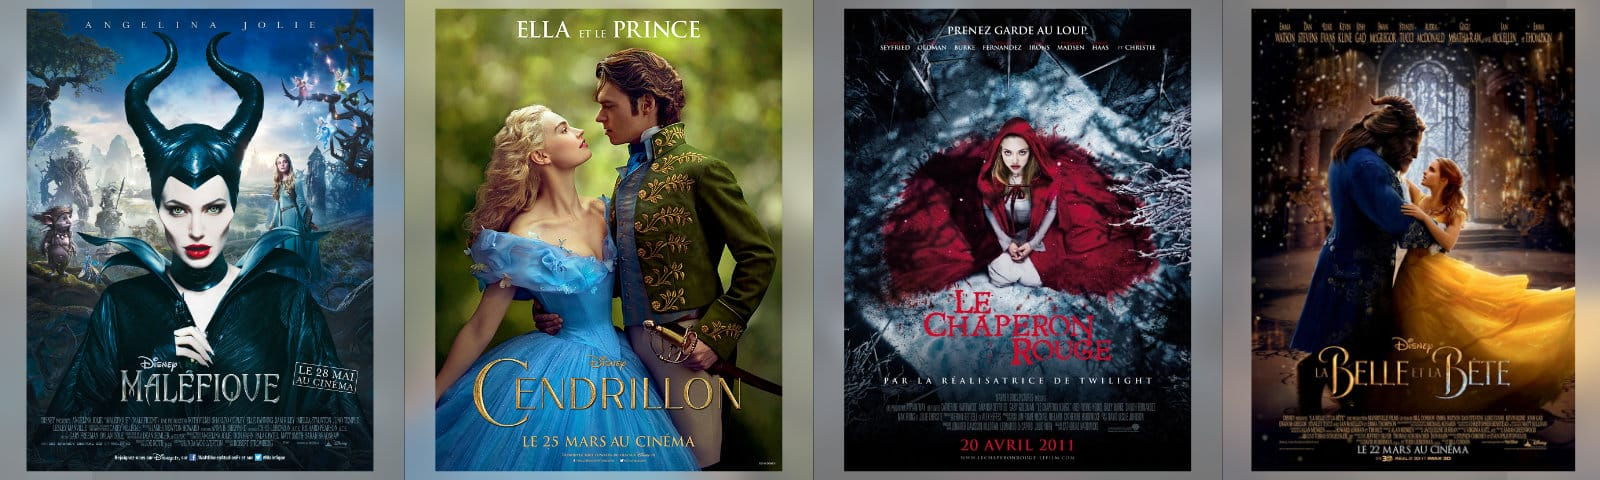
\includegraphics[width=1\textwidth,height=\textheight]{images/le-conte-ecrit-transpose-au-cinema.jpg}

\end{center}

La réalisation d'un film implique nécessairement une adaptation. Parfois les modifications apportées (titre, durée d'une action, lieux, les dialogues, enchaînements, etc.) sont telles que le film devient une œuvre nouvelle.
Il y a également une modification du point de vue du spectateur, dont la liberté interprétative est restreinte face à une mise en scène choisie.

\hypertarget{contes-et-leur-adaptation-cinuxe9matographique}{%
\subsection*{Contes et leur adaptation cinématographique}\label{contes-et-leur-adaptation-cinuxe9matographique}}
\addcontentsline{toc}{subsection}{Contes et leur adaptation cinématographique}

\begin{longtable}[]{@{}ll@{}}
\toprule
\begin{minipage}[b]{0.51\columnwidth}\raggedright
Conte\strut
\end{minipage} & \begin{minipage}[b]{0.43\columnwidth}\raggedright
Adaptation\strut
\end{minipage}\tabularnewline
\midrule
\endhead
\begin{minipage}[t]{0.51\columnwidth}\raggedright
La belle au bois dormant,\linebreak~Charles Perrault\strut
\end{minipage} & \begin{minipage}[t]{0.43\columnwidth}\raggedright
Maléfique\linebreak~(2014, Robert Stromberg)\strut
\end{minipage}\tabularnewline
\begin{minipage}[t]{0.51\columnwidth}\raggedright
Cendrillon,\linebreak~Charles Perrault\strut
\end{minipage} & \begin{minipage}[t]{0.43\columnwidth}\raggedright
Cendrillon\linebreak~(2015, Kenneth Branagh)\strut
\end{minipage}\tabularnewline
\begin{minipage}[t]{0.51\columnwidth}\raggedright
Le Petit Chaperon rouge,\linebreak~Charles Perrault\strut
\end{minipage} & \begin{minipage}[t]{0.43\columnwidth}\raggedright
Le Chaperon Rouge\linebreak~(2011, Catherine Hardwicke)\strut
\end{minipage}\tabularnewline
\begin{minipage}[t]{0.51\columnwidth}\raggedright
La Belle et la Bête,\linebreak~Jeanne-Marie Leprince de Beaumont\strut
\end{minipage} & \begin{minipage}[t]{0.43\columnwidth}\raggedright
La Belle et la Bête\linebreak~(2017, Bill Condon)\strut
\end{minipage}\tabularnewline
\bottomrule
\end{longtable}

\clearpage

Le sujet proposé vous permet d'explorer les différences entre un conte écrit et son adaptation cinématographique, à partir d'une thématique, d'un motif ou d'un autre point de comparaison. Pour ce faire, vous choisirez quelques extraits de texte au sein d'un conte afin de les mettre en parallèle avec les séquences du film correspondantes.

\begin{signature}
\emph{Suzanne Alves}

\end{signature}

\hypertarget{ruxe9uxe9criture-de-contes}{%
\chapter{Réécriture de contes}\label{ruxe9uxe9criture-de-contes}}

Depuis son émergence à la Renaissance, le genre du conte fascine. Usage du merveilleux, de héros et d'héroïnes charismatiques, motifs sociaux représentatifs d'une époque, distraction de l'auditoire à qui il est narré sont en vrac quelques éléments singuliers qui permettent de l'identifier. Il est d'ailleurs défini ainsi par Le dictionnaire du littéraire~:

\begin{quote}
``Le conte se caractérise par trois critères principaux~: il raconte des événements imaginaires, voire merveilleux~; sa vocation est de distraire, tout en portant souvent une morale~; il exprime une tradition orale multiséculaire et quasi universelle. D'abord «~populaire~» et oral, il est passé tôt en littérature lettrée {[}\ldots{]}, puis a donné toutes sortes de variantes''.\footnote{Aron, Paul, Saint-Jacques, Denis, Viala Alain (dir.), Le dictionnaire du littéraire, Paris, PUF, coll. «~Quadrige~», 2002, p.145 (les mises en gras sont de moi).}
\end{quote}

Ces variantes -- ou réécritures -- ont jalonné l'histoire du conte depuis son origine orale. Les collecteurs de contes, à l'image des frères Grimm (XVIII-XIXe), ont répertorié différentes versions des contes et ont contribué à ce passage de l'oral à l'écrit.

De nombreux contes ont été repris, modifiés, au fil du temps, pour correspondre davantage à la société dans laquelle ce récit évoluait. C'est le cas des versions Disney, expurgées des aspects choquants et violents des récits «~originels~» (par exemple la petite sirène d'Andersen se fait couper la langue par la sorcière des mers et a l'impression, durant son passage sur terre de marcher à chaque pas sur des couteaux aiguisés\ldots).

Ainsi, il existe d'innombrables versions des contes les plus célèbres, réécrites pour correspondre à l'époque dans laquelle il évolue. La dernière controverse en date est le baiser que donne le prince à la belle au bois dormant. Un baiser volé et non consenti, puisque le prince embrasse la belle sans son accord~; curieux pour ne pas dire dissonant dans une époque qui se veut égalitaire et où l'on proscrit l'abus de pouvoir du patriarcat.

Dans une époque mouvante comme la nôtre, peut-être est-il utile, sinon nécessaire, de proposer de nouvelles variantes de ces contes, adaptées à notre temps où les motifs, fussent-ils ancrés dans notre histoire, doivent être dépoussiérés et revisités pour correspondre à notre temps.

Ce travail de maturité entend répondre à cette question en mettant en évidence, d'une part, les motifs représentatifs d'un conte (aspect théorique) et en proposant une réécriture qui réinvestit ces mêmes motifs, mais à l'aune d'un éclairage actuel, une écriture 2.0 des Cendrillons, Belles au bois dormant et des Petites Sirènes\ldots{}

\begin{signature}
\emph{Pierre Bonjour et Samantha Steiner}

\end{signature}

\hypertarget{un-conte-et-des-conteurs}{%
\chapter{Un conte et des conteurs}\label{un-conte-et-des-conteurs}}

Saviez-vous que l'histoire de Barbe bleue est racontée au moins de trois façons différentes par les frères Grimm~? Connaissez-vous la première version de La Belle et la Bête, celle que Madame de Villeneuve avait composée et qui vous transportait bien plus loin dans les domaines du merveilleux et du féérique~? Avez-vous déjà lu le récit des souffrances de la petite sirène sous la plume de Hans Christian Andersen~? Ces contes qu'on croit connaître recèlent encore bien des mystères\ldots{}

Dans ce travail de maturité, vous étudierez différentes réécritures d'un conte de votre choix. Vous vous intéresserez aux changements qu'on découvre d'une version à l'autre et vous interrogerez quant à leur signification. Pourquoi ces variations~? Que révèlent-elles~? L'analyse peut porter sur des textes en anglais et en français. Il est également possible de choisir de rédiger le TM en anglais.

\begin{center}
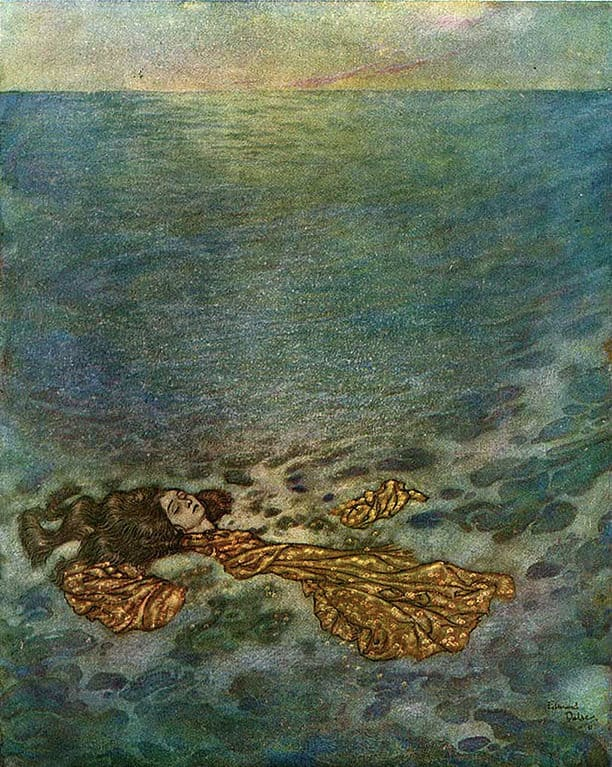
\includegraphics[width=\textwidth,height=12em]{images/un-conte-et-des-conteurs.jpg}

\end{center}

\begin{signature}
\emph{Samantha Steiner}

\end{signature}

\hypertarget{journaux-littuxe9rature-personnelle}{%
\chapter{Journaux (littérature personnelle)}\label{journaux-littuxe9rature-personnelle}}

Au fur et à mesure de l'histoire littéraire, les formes d'écriture de soi ont revêtu une myriade de formes différentes~: mémoires, autobiographies, autofictions, carnets, journaux intimes, etc. Dans tous les cas, il s'agit de s'exposer, de mettre en lumière un parcours, ponctuel (pensées du jour) ou diachronique (sur une partie ou l'ensemble d'une vie). Certaines de ces écritures de soi sont résolument personnelles, en témoignent les cadenas autour de certains carnets, d'autres, au contraire, s'adressent à un certain public pour qu'il ait accès à l'ensemble des rouages qui ont gouverné une vie.

Et s'il était possible de rendre accessibles les pensées d'un personnage historique (Napoléon, Jésus, etc.)~ou d'un personnage de fiction (Captain America, Aragorn, etc.)~? Dans ce travail, il s'agira de donner quelques éléments théoriques de l'écriture de soi, quelques éléments saillants qui reviennent systématiquement dans l'exposition de soi, dans un premier temps.

Dans un deuxième temps, il s'agira de sélectionner un personnage emblématique et de coucher sur le papier les pensées, dilemmes, interrogations qu'il aurait dû avoir à un moment de sa vie\ldots{}

Ce travail se veut créatif, et, hormis la contrainte de l'écriture de soi (ici, l'écriture d'un autre soi, imaginaire et fantasmé), l'élève est libre de choisir un personnage réel ou fictif et de rédiger un ensemble de pensées originales qui auraient pu survenir sous la plume dudit personnage.

\begin{signature}
\emph{Pierre Bonjour}

\end{signature}

\hypertarget{les-machines-et-la-communication-outils-et-sensibilituxe9s}{%
\chapter{\texorpdfstring{Les machines et la communication : \linebreak outils et sensibilités}{Les machines et la communication : outils et sensibilités}}\label{les-machines-et-la-communication-outils-et-sensibilituxe9s}}

\begin{center}

\includegraphics[width=\textwidth,height=12em]{images/les-machines-et-la-communication.jpg}

\end{center}

\begin{center}
\textbf{``Dis Siri : Veux-tu m'épouser~?''}\\
\textbf{``Dis Siri : Est-ce que tu m'aimes~?''}

\end{center}

Il parait que ce sont là les questions le plus souvent posées à cette application vocale.

L'être humain est un animal social pour qui communiquer est vital. Comme ``on ne peut pas ne pas
communiquer''\footnote{WATZLAWICK, P., BEAVIN-BAVELAS, J., \& JACKSON, D. (1972) : Une logique de la communication, Éd. du Seuil, Paris}, tout est communication.

Comment communique-t-on ? Par quels canaux ? La tentation de répondre ``par le langage'' en premier est grande alors que les études ont montré que lors d'un échange de type ``face-à-face'', la communication verbale ne représenterait que 7\% \ldots{}

Que se passe-t-il quand on ``communique'' avec Siri ? Les êtres humains emploient le langage naturel qui est différent du langage formel comme les mathématiques ou différents langages informatiques. Le traitement automatique du langage naturel (TALN), discipline de l'intelligence artificielle (IA) se consacre aux interactions entre l'humain et les machines. Eh oui, même si Siri nous répond à des questions plus ou moins loufoques, lui et nous, nous ne parlons pas le même langage. Mais qui parle quoi, alors ?

Le TALN a également permis de nouvelles percées dans le monde des communications multilingues. Les solutions de traduction automatique en ligne sont maintenant des outils accessibles à tous. Associé à la reconnaissance automatique de la parole, le TALN permet à des personnes de langues différentes de communiquer entre elles.

Mais il y a traduire et \ldots traduire ou, selon l'expression consacrée, ``traduire c'est trahir'' qui renvoie à la différence irréductible entre un texte et ses traductions possibles. Quel rôle les technologies de traduction automatique jouent-elles non seulement dans notre vie quotidienne, à l'école et au travail, mais aussi dans la recherche scientifique et les études littéraires ? Est-il possible de confier à DeepL la traduction d'un texte de loi ou d'un poème de Goethe ?

De quoi est-elle donc capable l'IA aujourd'hui ? Quel est l'état actuel des connaissances et quels progrès seraient envisageables ? Voici quelques-unes des questions qui pourraient être le point de départ de travaux de maturité axés sur la communication humaine naturelle, artificielle, mixte, mono ou multilingue.

Les trois enseignantes responsables sont plurilingues et se prêtent à des expérimentations en plusieurs langues : français, roumain, portugais, anglais, allemand et italien.

Les travaux peuvent être rédigés en français et en allemand.

\begin{signature}
\emph{Eugenia Portioli}\\
\emph{Carla Bastos}\\
\emph{Anamaria Terrier}

\end{signature}

\hypertarget{repruxe9sentations-des-figures-huxe9rouxefques-ou-non-dans-les-bandes-dessinuxe9es-dc-marvel-mangas}{%
\chapter{\texorpdfstring{Représentations des figures héroïques \linebreak (ou non) dans les bandes dessinées \linebreak (DC, Marvel, mangas \ldots)}{Représentations des figures héroïques (ou non) dans les bandes dessinées (DC, Marvel, mangas \ldots)}}\label{repruxe9sentations-des-figures-huxe9rouxefques-ou-non-dans-les-bandes-dessinuxe9es-dc-marvel-mangas}}

\begin{center}
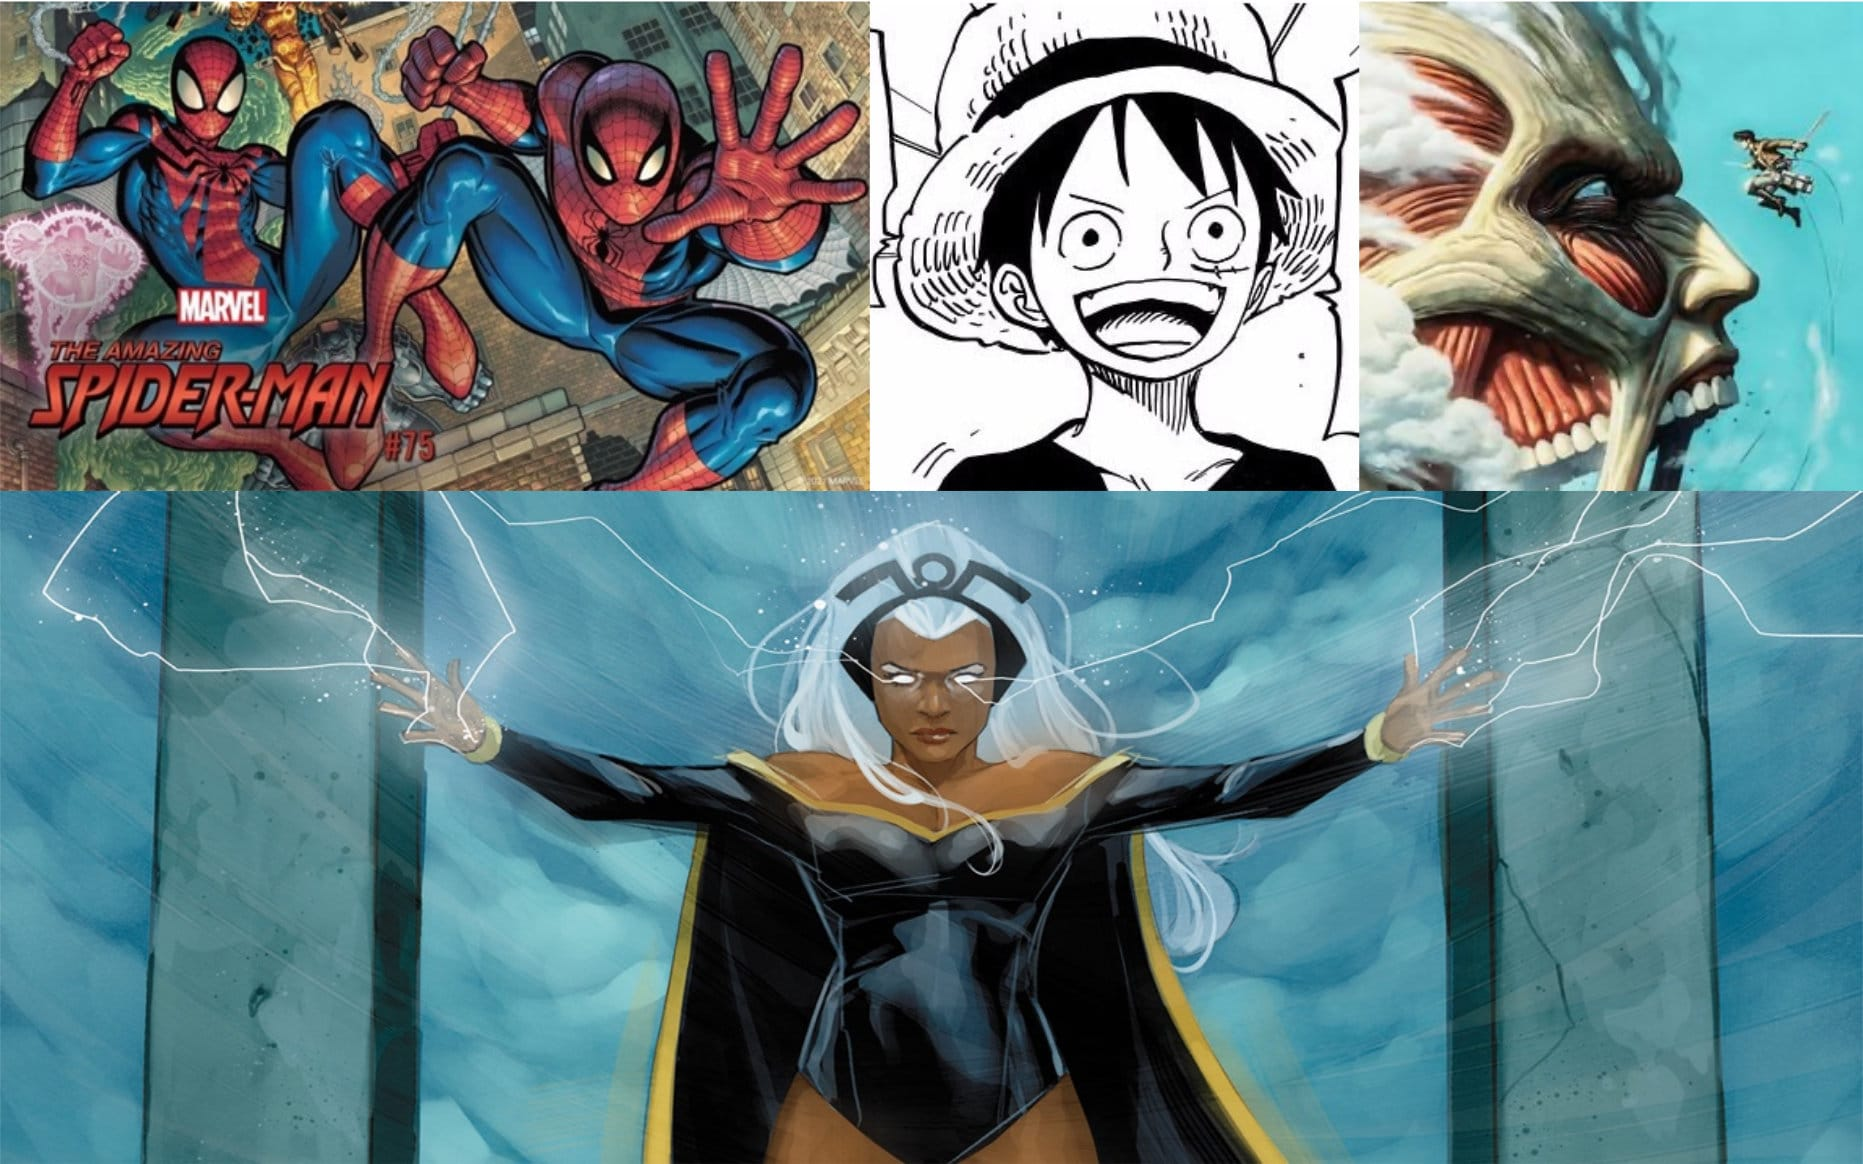
\includegraphics[width=\textwidth,height=12em]{images/representations-des-figures-heroiques.jpg}\\
\footnote{Images : LEE, S., DITKO, S.: The Amazing Spider-Man; ODA, E.: One Piece ; ISAMAYA, H.: Attack on Titan; WEIN, L., COCKRUM, D.: X-Men.}

\end{center}

Avez-vous déjà rêvé d'être piqué par une araignée et de devenir le nouveau Peter Parker ? Imaginez-vous parfois que vous pouvez contrôler le vent telle Tornade ? Enviez-vous le chapeau de paille du personnage loufoque et pas toujours héroïque de Luffy ? Craignez-vous d'être un titan enfermé, comme Eren Jäger, dans un paradis fictif ? Ou que la réalité que nous connaissons ne soit qu'un mensonge~?

Depuis l'Iliade d'Homère jusqu'aux personnages de l'univers Marvel en passant par le roi Arthur et le monde des mangas, les figures du héros et de l'anti-héros passionnent et interrogent. Au travers de ce travail de maturité, il s'agira d'explorer ces notions et d'analyser les traits caractéristiques de la figure héroïque ou antihéroïque dans les bandes dessinées et les adaptations cinématographiques. Que représentent ces personnages~? Qu'est-ce qui est constitutif d'un héros ou d'une héroïne~? Quelle est la place accordée aux figures féminines dans les représentations actuelles~? Peut-on réduire la figure de l'anti-héros à un simple antagoniste ou au «~méchant~» de l'histoire ? Dans quelle mesure le contexte historique justifie ou explique-t-il l'évolution de ces figures~? Telles pourraient être les questions abordées dans le cadre de cette thématique.

Ce travail de maturité doit être rédigé en binôme. Il peut être rédigé en français, en anglais ou en allemand.

\begin{signature}
\emph{Swaha Somanadan}\\
\emph{Pauline Meylan}\\
\emph{Eugenia Portioli}

\end{signature}

\hypertarget{uxe9laboration-dun-guide-de-voyage-dans-une-ville-germanophone}{%
\chapter{Élaboration d'un guide de voyage dans une ville germanophone}\label{uxe9laboration-dun-guide-de-voyage-dans-une-ville-germanophone}}

\begin{center}
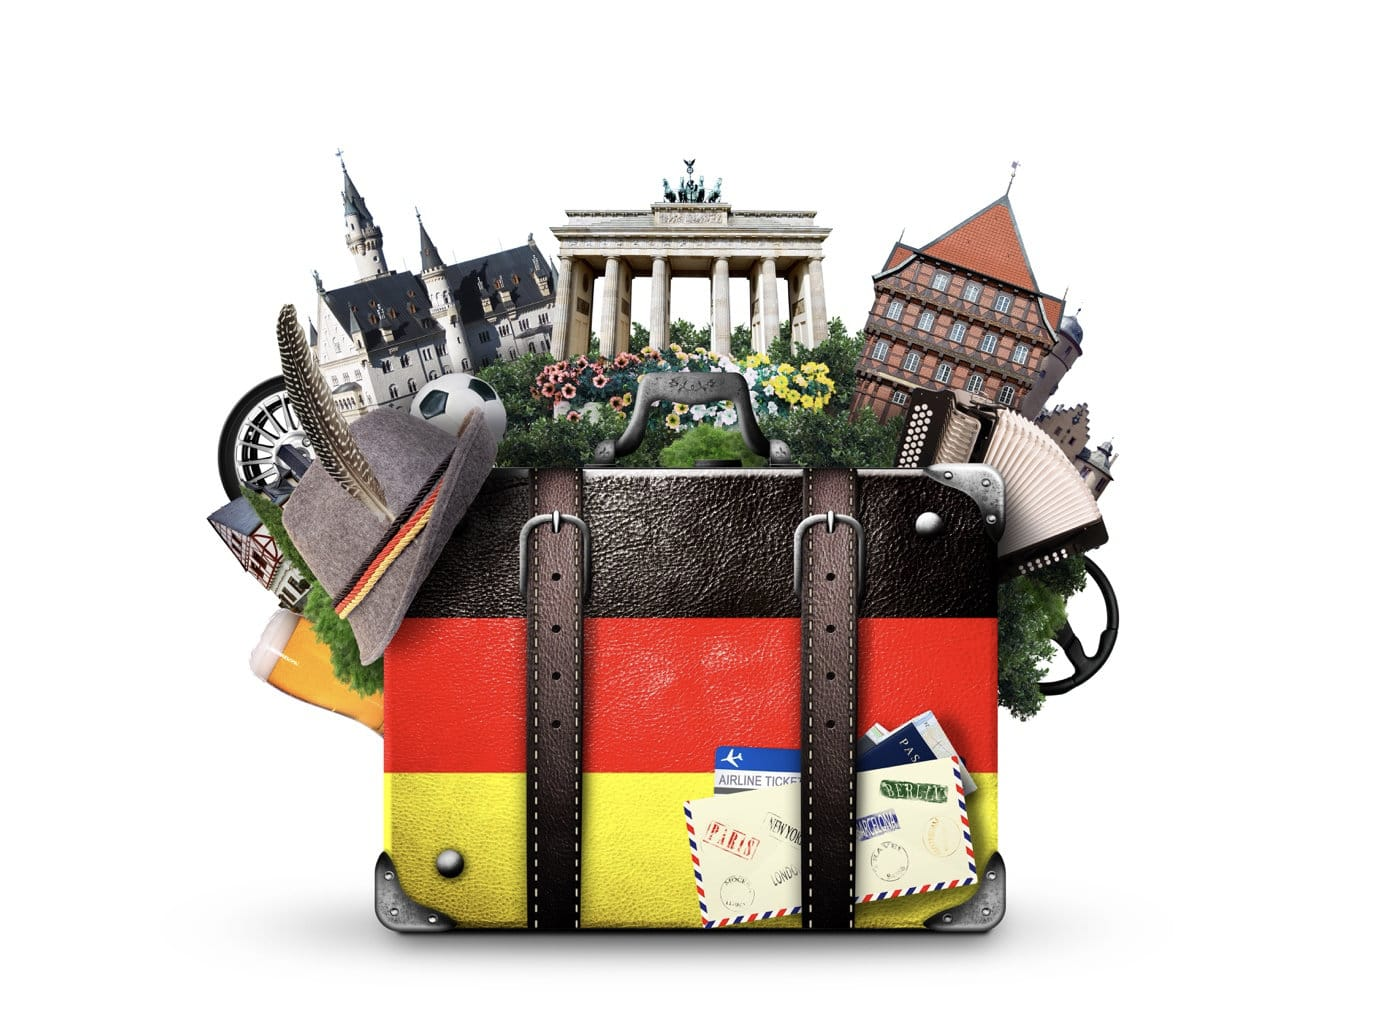
\includegraphics[width=\textwidth,height=12em]{images/elaboration-dun-guide-de-voyage.jpg}

\end{center}

Un guide touristique est déjà une invitation au voyage~: les images nous transportent dans des endroits reculés, la mise en page emmène le lecteur sur les histoires des lieux à visiter, les polices de caractère révèlent la personnalité du texte. Tant de qualités avec lesquelles jouer~!

Qui aurait envie de visiter Vienne muni d'un guide sans images, qui aurait envie de lire l'histoire de St-Gall dans un bloc texte sans paragraphes, enfin qui aurait l'usage d'un guide de Berlin sans carte de métro ?

Graphiquement, le guide est un livre fait d'images, de texte et des cartes. Concrètement, il s'agit d'un objet petit et pratique. Une partie de ce TM consiste à fabriquer un exemplaire de votre guide touristique.

Tout comme la forme, le contenu du guide est aussi essentiel. Il doit être précis et efficace. Tous les aspects d'un voyage devraient être abordés~: culture, logement, restaurant, transport et bien d'autres thématiques encore selon vos envies.

Dans le cadre de ce TM, la culture germanophone est au centre. Aber keine Panik~! Ce projet s'adresse à vous qui adorez voyager et créer, même si la langue allemande n'est pas votre tasse de thé. L'idée est de découvrir et de faire découvrir une ville en Allemagne, en Autriche ou en Suisse Alémanique et d'en élaborer un petit guide touristique à l'attention d'autres étudiants. Il peut être rédigé en français ou en allemand~: c'est vous qui voyez.

\begin{signature}
\emph{Stéphanie Macrina}

\end{signature}

\hypertarget{le-ruxe9cit-de-voyage}{%
\chapter{Le récit de voyage}\label{le-ruxe9cit-de-voyage}}

\begin{center}
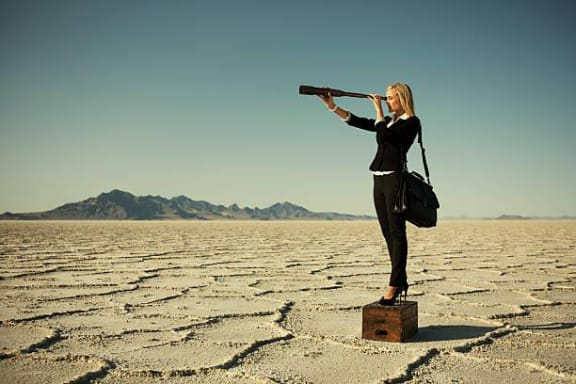
\includegraphics[width=\textwidth,height=12em]{images/le-recit-de-voyage.jpg}

\end{center}

De tous temps, nous, humains, avons ressenti l'appel du large et sommes partis à l'aventure vers des contrées inconnues pour en rapporter des histoires fantastiques. Le voyage permet de sortir de nos habitudes, de retrouver l'essentiel et parfois de nous donner l'illusion de la liberté.

Dans ce TM il s'agira de choisir votre propre destination pour ensuite en faire un récit de voyage. Nous aborderons le récit de voyage à travers des auteurs comme Sylvain Tesson, Ella Maillart ou d'autres écrivains. Puis ça sera à vous, par groupe de deux, d'organiser puis d'entamer votre voyage qui constituera la base de votre récit. Nul besoin d'aller à l'autre bout de la planète : il s'agit de sortir de son quotidien et de sa zone de confort et de partir à la découverte de lieux nouveaux qui nourrissent notre imaginaire. Vous en ferez ensuite votre propre récit de voyage, un texte écrit et agrémenté par exemple de photos, de vidéos ou de dessins pour à votre tour faire voyager vos lecteurs.

N.B. Ce TM peut se faire en français ou en anglais et doit être rédigé à deux.

\hypertarget{travel-literature}{%
\section*{Travel literature}\label{travel-literature}}
\addcontentsline{toc}{section}{Travel literature}

For ages, we have felt the call from the sea and have adventured towards unknown places coming back to narrate our incredible experiences. Traveling allows us to escape from our habits, find what's essential and sometimes gives us the illusion of being free.

In this TM you will discover what travel literature is, through texts by Sylvain Tesson, Ella Maillart or other writers. Then it will be your turn, in groups of two, to organise and start off your own travel adventure which will be the starting point of your text. No need to go far away: it's about leaving our daily routine and comfort zone to discover new places that fuel our imagination. You will then produce a written text on your travel adding for example photos, videos and drawings to make your readers travel as well.

N.B. This TM can be written in French or English and needs to be done in groups of two.

\begin{signature}
\emph{Jasmine Menamkat}

\end{signature}

\hypertarget{multiculturalituxe9-et-langage}{%
\chapter{Multiculturalité et langage}\label{multiculturalituxe9-et-langage}}

\begin{center}
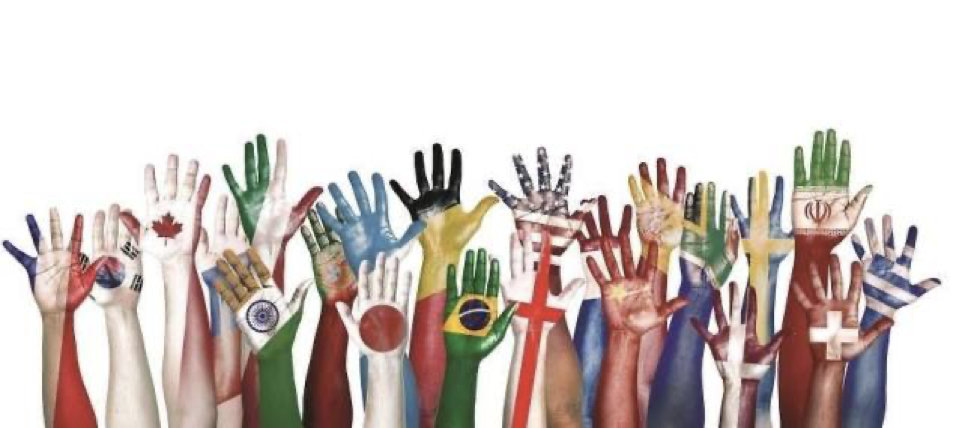
\includegraphics[width=\textwidth,height=12em]{images/multiculturalite-et-langage.jpg}\\
\footnote{Image : \url{https://multiulb.com/finalite-multiculturalite/}}

\end{center}

Dans un monde globalisé et souvent polarisé, il est parfois aussi difficile d'aller à la rencontre de l`Autre que de vivre pleinement sa propre culture. Avoir des origines multiculturelles peut même être source de difficultés, malentendus, voire de conflits.

Ce travail s'adresse avant tout aux élèves qui vivent au quotidien une situation inter- (ou multi-) culturelle: enfants de parents de différentes nationalités, religions, origines; étrangers en Suisse, enfants adoptés, Suisses de retour de l'étranger.
Il est aussi ouvert à celles et ceux qui s'intéressent à la diversité culturelle, et souhaiteraient décortiquer quelques stéréotypes et préjugés.

Chaque participant·e sera invité à définir une problématique qui résulte de sa situation personnelle ou observée (problème d'intégration, discrimination raciale, différence de mentalité, difficultés linguistiques, contraintes vestimentaires ou alimentaires, etc.)

Les participant·e·s pourront aussi se pencher sur les rites et traditions liés à une culture, et la difficulté ---ou la pertinence--- de les préserver dans le monde actuel. Les notions d'~``appropriation culturelle'' et d'héritage colonial pourraient également être explorées, de même que le concept d'une Europe unie (UE) face aux idées indépendantistes et séparatistes.

Chacun·e tâchera ensuite de considérer son sujet sous divers angles et perspectives. Le travail en duo devrait offrir une symétrie et complémentarité d'analyse.

En dernier lieu, il s'agira de proposer des solutions et des ouvertures.

Une introduction à la communication interculturelle sera proposée à travers une série de lectures sur le sujet (E. Hall, etc.). Lors de la semaine spéciale, des rencontres avec des invité·e·s (expert·e·s ou témoins) seront organisées.

Le choix de langue de rédaction et de forme (étude scientifique, enquête journalistique, texte créatif, reportage, etc.) sera discuté avec le ou la répondant·e.

\begin{signature}
\emph{Suzanne Alves} (français, espagnol, portugais)\\
\emph{Joel Atakora} (français, allemand, suisse-allemand, média)\\
\emph{Beata Jaquet} (anglais, espagnol, français, polonais, Europe de l'Est)\\
\emph{Esma Puric} (italien, philosophie-psychologie,\\
langue et culture bosniaque)\\
\emph{Valentina Sacco} (italien, français)

\end{signature}

\hypertarget{les-nombres-remarquables}{%
\chapter{Les nombres remarquables}\label{les-nombres-remarquables}}

En mathématiques, il y a des nombres qui se distinguent des autres par leurs propriétés étonnantes ou leur rôle clé dans une ou plusieurs branches des mathématiques. On les appelle les nombres remarquables.
Peut-on imaginer de faire les mathématqiues sans le zéro~? Que serait la trigonométrie sans la constante d'Archimède π~? Qui ne pense pas quand on parle des nombres complexes à ce nombre imaginaire si particulier dont le carré est égal à . Les nombres 0, π et sont des exemples de nombres remarquables.

\begin{center}
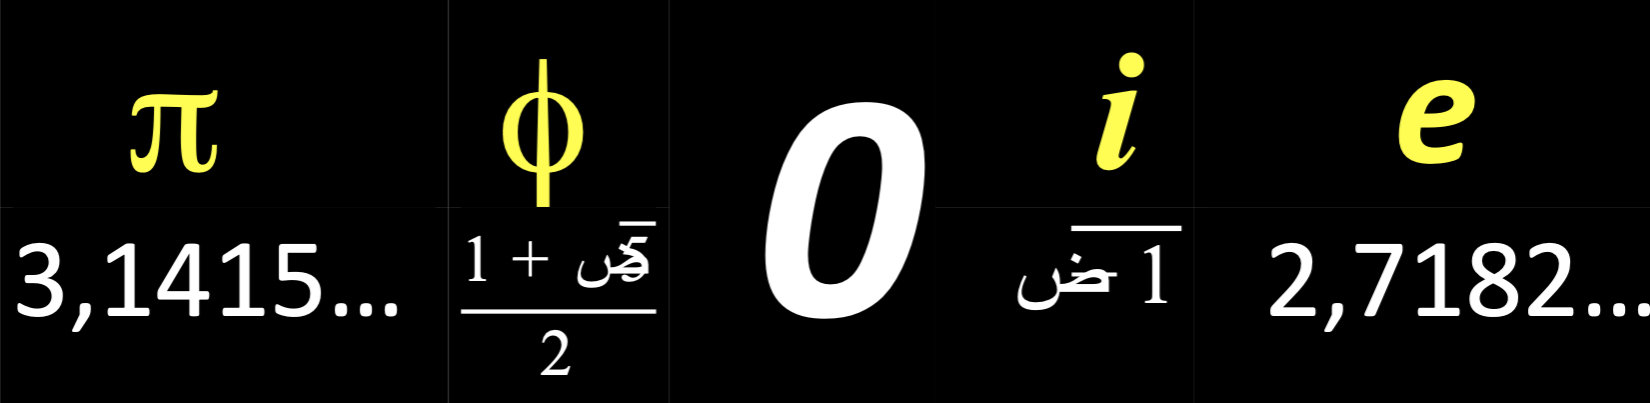
\includegraphics[width=\textwidth,height=12em]{images/les-nombres-remarquables-1.jpg}

\end{center}

Il existe d'autres nombres remarquables. Par exemple le nombre appelé le nombre d'Euler ou la constante de Néper est central pour l'étude de l'exponentielle en base et du logarithme naturel. Il existe également des familles de nombres remarquables comme les nombres premiers qui sont des nombres entiers naturels ayant exactement deux diviseurs positifs 1 et eux-mêmes. Parmi les nombres premiers, 2 a la particularité d'être le seul nombre pair qui est premier. Parmi les nombres remarquables certains portent des noms curieux comme les nombres déficients, les nombres abondants, les nombres amiables ou les nombres univers.

\begin{center}
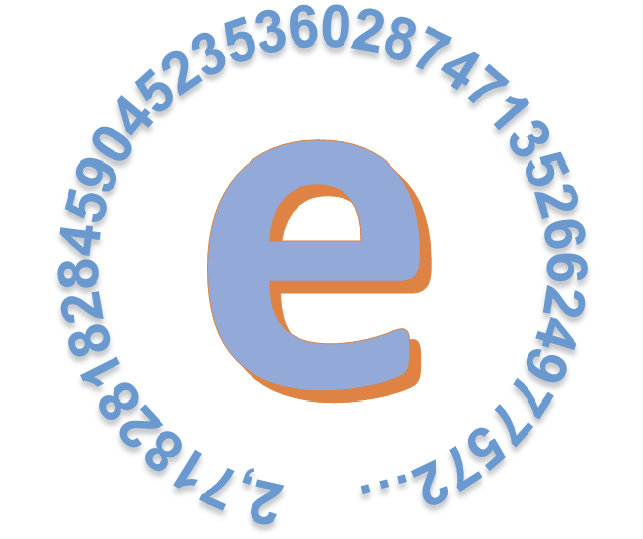
\includegraphics[width=\textwidth,height=12em]{images/les-nombres-remarquables-2.jpg}

\end{center}

Ce thème propose aux candidats intéressés de travailler sur un nombre remarquable ou une famille de nombres remarquables afin d'explorer leurs caractéristiques et leurs propriétés fondamentales et d'étudier leur importance en mathématiques ainsi que leurs applications dans différents domaines.

\begin{signature}
\emph{Carla Bastos Da Silva}\\
\emph{Ahmed Bufardi}\\
\emph{Yannick Donnet}\\
\emph{Frédéric Makiadi}\\
\emph{Alan Morier}

\end{signature}

\hypertarget{la-guxe9omuxe9trie-non-euclidienne}{%
\chapter{La géométrie non euclidienne}\label{la-guxe9omuxe9trie-non-euclidienne}}

\begin{center}
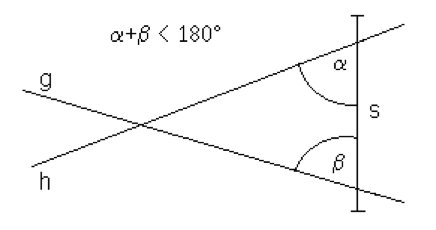
\includegraphics[width=\textwidth,height=9em]{images/la-geometrie-non-euclidienne-1.jpg}\\
\footnote{Par Phrontis --- Travail personnel, CC BY 3.0, \url{https://commons.wikimedia.org/w/index.php?curid=7618684}}

\end{center}

La géométrie euclidienne, celle que vous connaissez, repose sur cinq axiomes et cinq postulats. Citons le cinquième postulat~: ``Si une droite, tombant sur deux droites, fait les angles intérieurs du même côté plus petits que deux angles droits, ces droites, prolongées à l'infini, se rencontreront du côté où les angles sont plus petits que deux angles droits''. Ils permettent d'en déduire des propriétés bien connues, comme par exemple~: la somme des angles d'un triangle vaut 180 °.

Durant des siècles, les mathématiciens ont essayé de prouver que le cinquième postulat n'était pas nécessaire pour construire la géométrie euclidienne, sans succès. Nous comprendrons plus tard qu'il n'est pas possible de s'en séparer. Mais si nous l'enlevons, nous pouvons obtenir des nouvelles géométries, appelées ``géométries non euclidienne''. Les plus connues sont la géométrie sphérique et la géométrie hyperbolique.

\begin{center}
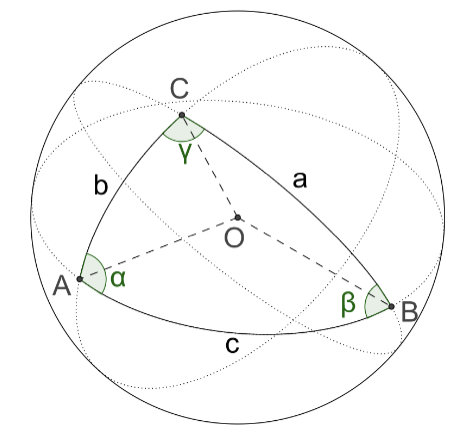
\includegraphics[width=\textwidth,height=9em]{images/la-geometrie-non-euclidienne-2.jpg}\\
\footnote{Par HB --- Travail personnel, CC BY-SA 4.0, \url{https://commons.wikimedia.org/w/index.php?curid=71758828}}

\end{center}

Dans la géométrie sphérique, nous étudions les objets géométriques dans une sphère. Sur la figure ci-dessus, vous pouvez voir un triangle en géométrie sphérique. Ici, la somme des angles un triangle est supérieure à 180°. Cette géométrie est utilisée entre autres dans la cartographie.

\begin{center}
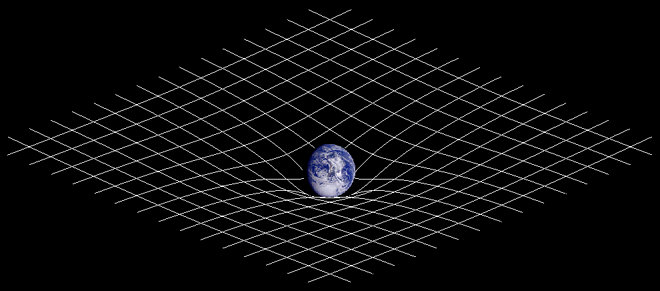
\includegraphics[width=\textwidth,height=9em]{images/la-geometrie-non-euclidienne-3.jpg}\\
\footnote{Source : Par Johnstone sur Wikipédia anglaisTexte original : Created by User Johnstone using a 3D CAD software package and an image of planet earth from NASA's Galileo spacecraft. --- Travail personnel, CC BY-SA 3.0, \url{https://commons.wikimedia.org/w/index.php?c}}

\end{center}

Dans la géométrie hyperbolique, nous étudions les objets géométriques dans un hyperboloïde. Cette fois, la somme des angles d'un triangle sera inférieure à 180°. Nous utilisons cette géométrie notamment dans l'astronomie. Une planète, avec sa masse, va courber l'espace-temps et lui donner la forme d'un hyperboloïde. Si un objet passe à proximité ce cette planète, sa trajectoire sera donc courbée.

\clearpage

Dans ce TM, nous vous proposons d'étudier l'une des deux géométries et de l'appliquer à un cas concret, ou de comparer la géométrie euclidienne et une géométrie non euclidienne.

\begin{signature}
\emph{Carla Bastos Da Silva}\\
\emph{Ahmed Bufardi}\\
\emph{Yannick Donnet}\\
\emph{Frédéric Makiadi}\\
\emph{Alan Morier}

\end{signature}

\hypertarget{les-duxe9fis-de-lalimentation}{%
\chapter{Les défis de l'alimentation}\label{les-duxe9fis-de-lalimentation}}

\begin{center}
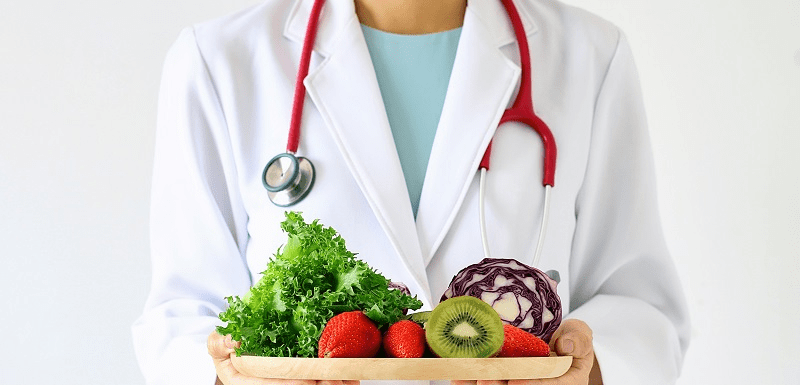
\includegraphics[width=\textwidth,height=12em]{images/les-defis-de-lalimentation.png}

\end{center}

De quoi parle-t-on lorsqu'on aborde l'alimentation ? De gastronomie~? De santé et de diététique ? De tradition et de patrimoine ? De production et d'échanges de nourriture ? De règles alimentaires et de dogmes~?

Il y a 50~ans, on concevait encore l'alimentation comme allant de soi. Récemment, différents facteurs ont contribué à modifier notre perception de cette dernière.

A travers ce TM, je vous invite à découvrir le monde de l'alimentation à travers le regard d'un scientifique et d'en savoir plus sur ses défis d'hier, d'aujourd'hui et de demain. ~

Voici quelques exemples non exhaustifs de champs d'études possibles :

\begin{itemize}
\tightlist
\item
  L'anthropologie alimentaire s'intéresse à l'ensemble des activités de production, de transformation, de distribution et de consommation alimentaires et aux pratiques et aux représentations qui s'y rattachent. Cela peut comporter l'étude de différents modes de conservation et leurs impacts sur la qualité nutritionnelle des aliments, des recherches biomédicales qui font le lien entre les habitudes alimentaires et certaines maladies, ou de l'adaptation de l'humain face à des contraintes nutritionnelles.
\item
  L'épidémiologie nutritionnelle se focalise sur les maladies épidémiologiques en lien avec la nutrition.
\item
  La nutrition se concentre quant à elle aux rôles des nutriments dans l'organisme humain et à leurs interactions ainsi qu'aux besoins nutritionnels des individus et des populations.
\end{itemize}

Les travaux de maturité dans cette thématique se feront obligatoirement par binôme.

\begin{signature}
\emph{Sophie Guernier}

\end{signature}

\hypertarget{uxe9tude-de-la-biodiversituxe9}{%
\chapter{Étude de la biodiversité}\label{uxe9tude-de-la-biodiversituxe9}}

\begin{center}
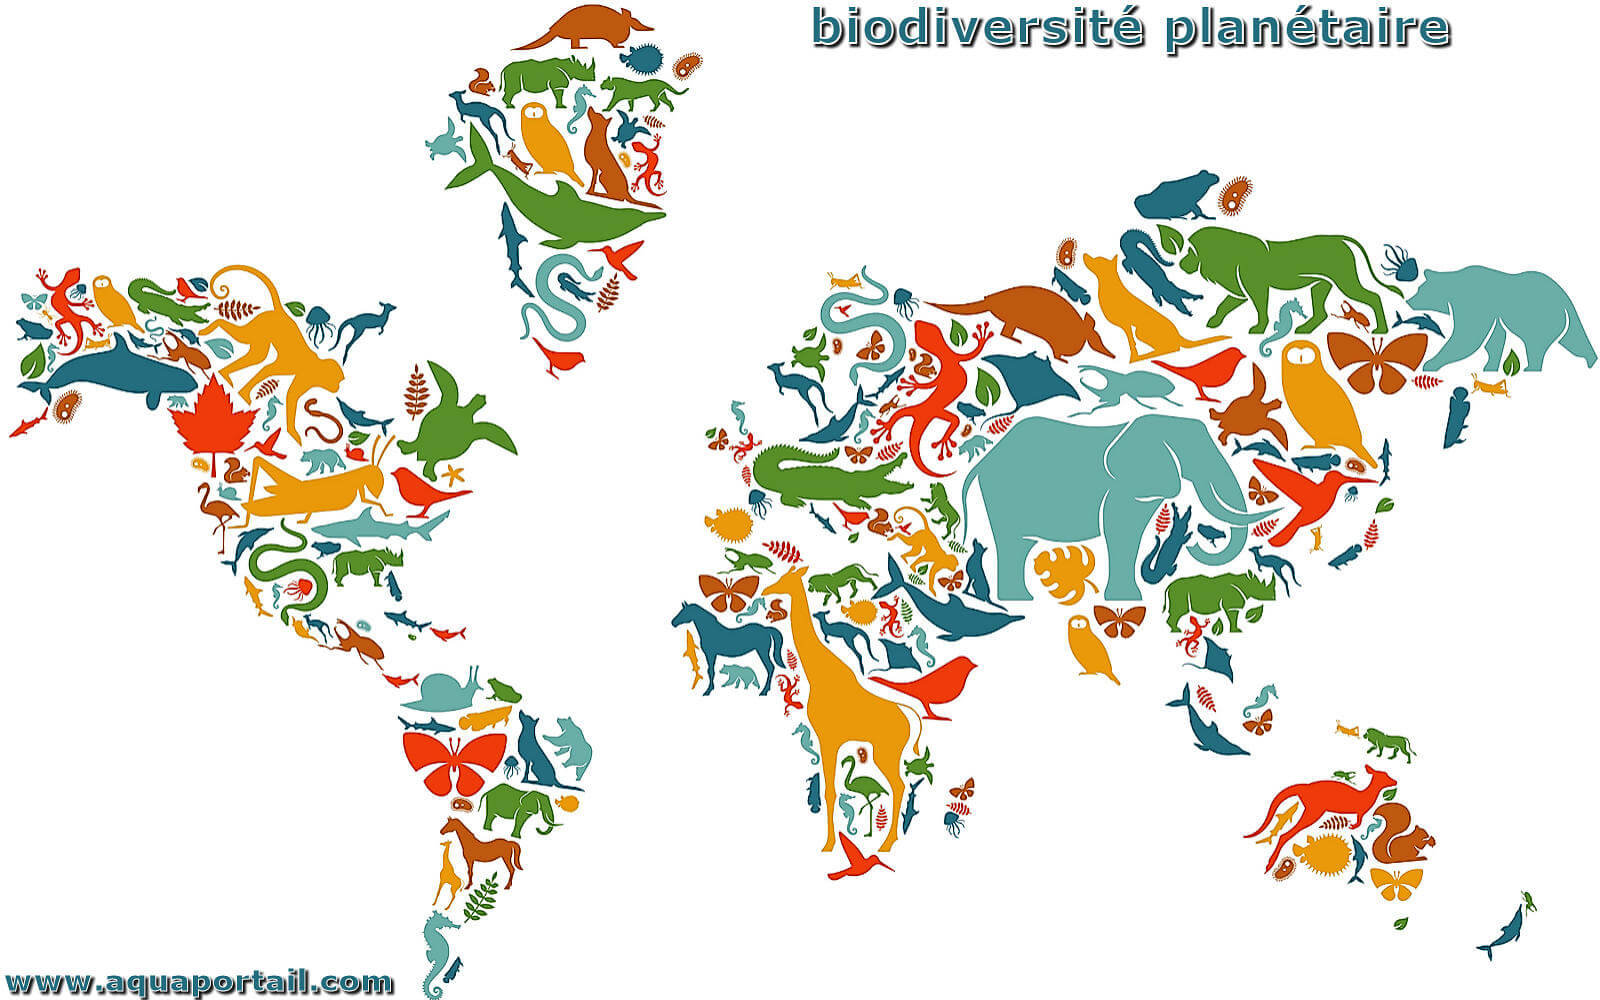
\includegraphics[width=\textwidth,height=12em]{images/etude-de-la-biodiversite.jpg}

\end{center}

L'un des plus grands défis auxquels l'humanité est actuellement confrontée est la perte de la biodiversité au niveau planétaire. Celle-ci est causée par différents processus, par exemple la déforestation massive qui amène à la perte d'habitat, le réchauffement climatique qui détruit des écosystèmes et en modifie d'autre.

Afin de pouvoir inverser et atténuer la perte de biodiversité et ses conséquences, il est indispensable de mieux connaitre et mieux recenser la biodiversité de nos régions pour mesure ces impacts.

A travers ce TM, je vous invite à réaliser une étude de la biodiversité afin de mieux appréhender cette méthodologie. A vous de décider de la suite de ce TM en fonction du site d'étude (forêt, lac, tronc d'arbre mort\ldots{} ), de l'espèce ou des espèces à analyser (oiseaux migrateurs, fourmis, plantes invasives), de la façon de répertorier la biodiversité de façon directe ou indirecte.

Les travaux de maturité en lien avec cette thématique se feront obligatoirement par binôme.

\begin{signature}
\emph{Sophie Guernier}

\end{signature}

\hypertarget{lintelligence-artificielle-est-elle-vraiment-intelligente}{%
\chapter{\texorpdfstring{L'intelligence artificielle \linebreak est-elle vraiment intelligente~?}{L'intelligence artificielle est-elle vraiment intelligente~?}}\label{lintelligence-artificielle-est-elle-vraiment-intelligente}}

\begin{center}
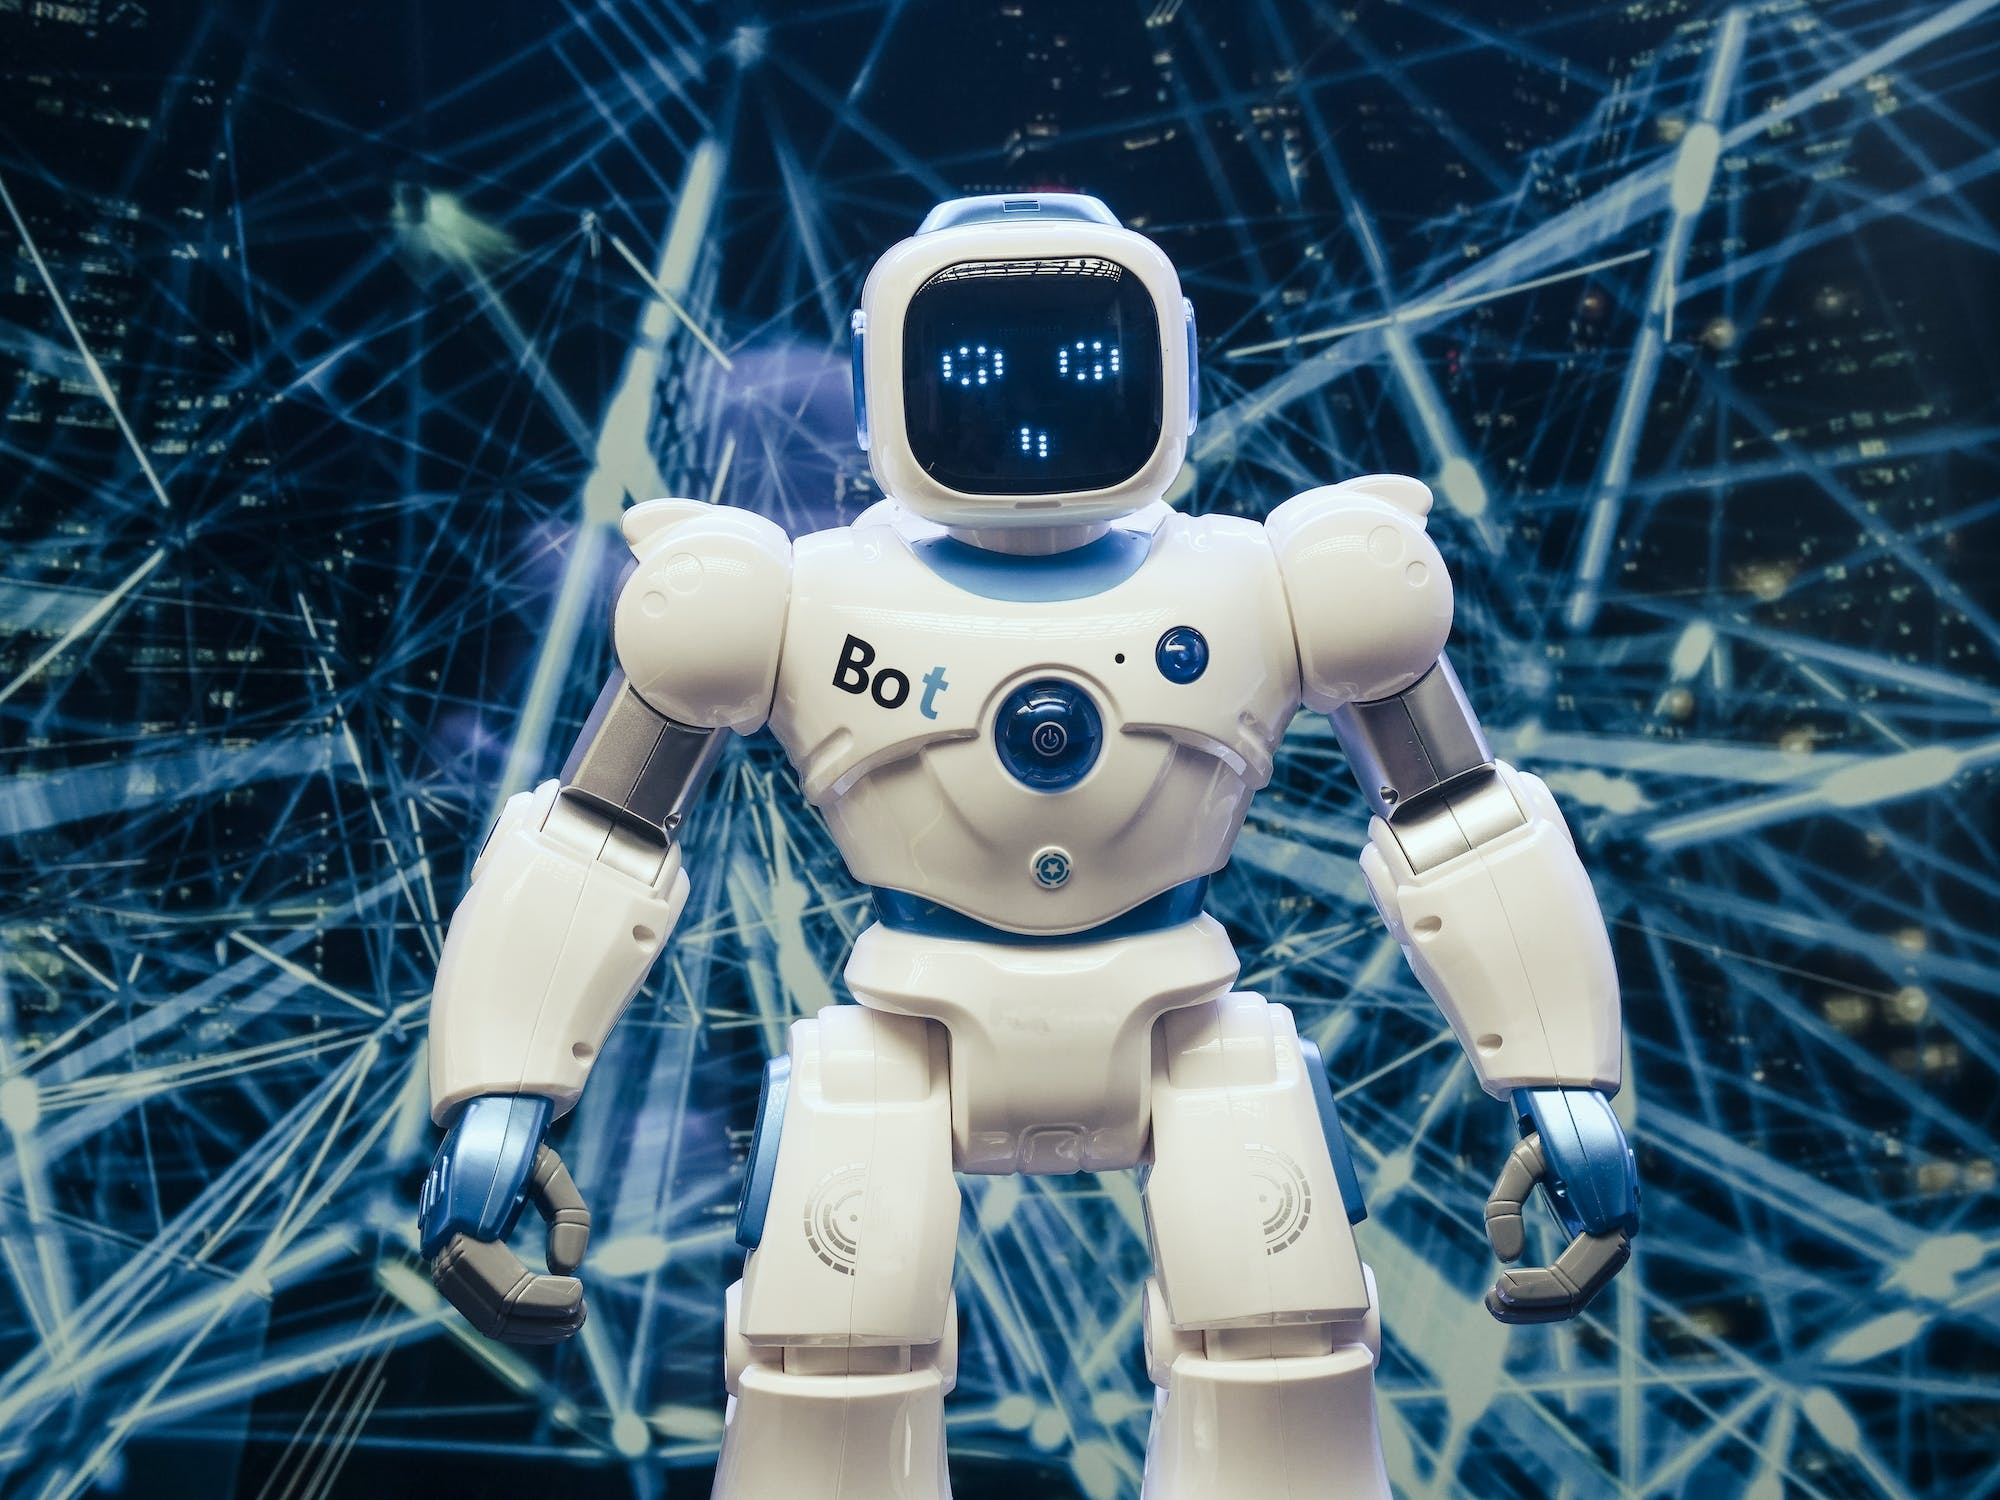
\includegraphics[width=\textwidth,height=12em]{images/intelligence-artificelle.jpeg}

\end{center}

\hypertarget{une-machine-peut-elle-reproduire-les-fonctions-cognitives-avancuxe9es-tel-que-la-pensuxe9e-humaine}{%
\subsection*{Une machine peut-elle reproduire les fonctions cognitives avancées tel que la pensée humaine~?}\label{une-machine-peut-elle-reproduire-les-fonctions-cognitives-avancuxe9es-tel-que-la-pensuxe9e-humaine}}
\addcontentsline{toc}{subsection}{Une machine peut-elle reproduire les fonctions cognitives avancées tel que la pensée humaine~?}

La question de savoir si l'humain par ces caractéristiques est unique dans le monde du vivant a été soulevée bien avant l'arrivée des machines. Aujourd'hui se pose également la question de savoir si l'humain est unique par ces capacités cognitives notamment face aux machines dotées d'intelligence artificielle.

Au moins depuis 1950, lorsque M. Turing publie un premier article sur l'apprentissage machine et l``'intelligence artificielle'' \footnote{Turing, A. M. (1950). I.---COMPUTING MACHINERY AND INTELLIGENCE. Mind, LIX(236), 433-460.}, s'est ouvert le débat de savoir si une machine pouvait reproduire les fonctions cognitives avancées tels que la pensée humaine.

De nos jours, des machines dites intelligentes rivalisent avec de plus en plus de succès avec les humains pour des tâches autrefois considérées comme hors de portée de l'intelligence artificielle. On peut notamment penser à la reconnaissance d'images ou de vidéos d'objets et de visages, à la capacité à répondre à des questions posées en langage ``naturel'' par un humain (robots répondeurs), voir même dans certains cas de prendre des décisions dites stratégiques dans des conditions de risque et d'incertitude. On peut également citer les vidéos modifiées par intelligence artificielle pour lesquelles il peut être difficile de déceler le ``vrai'' du ``faux''.

Les machines sont donc capables de nombreuses prouesses, mais sont-elles vraiment intelligentes~? Sont-elles capables de reproduire les fonctions cognitives avancées tel que la pensée humaine ? Votre travail de maturité pourrait aborder ces questions.

\begin{signature}
\emph{Manuel Zenger}

\end{signature}

\hypertarget{santuxe9-et-sport}{%
\chapter{Santé et sport}\label{santuxe9-et-sport}}

\begin{center}
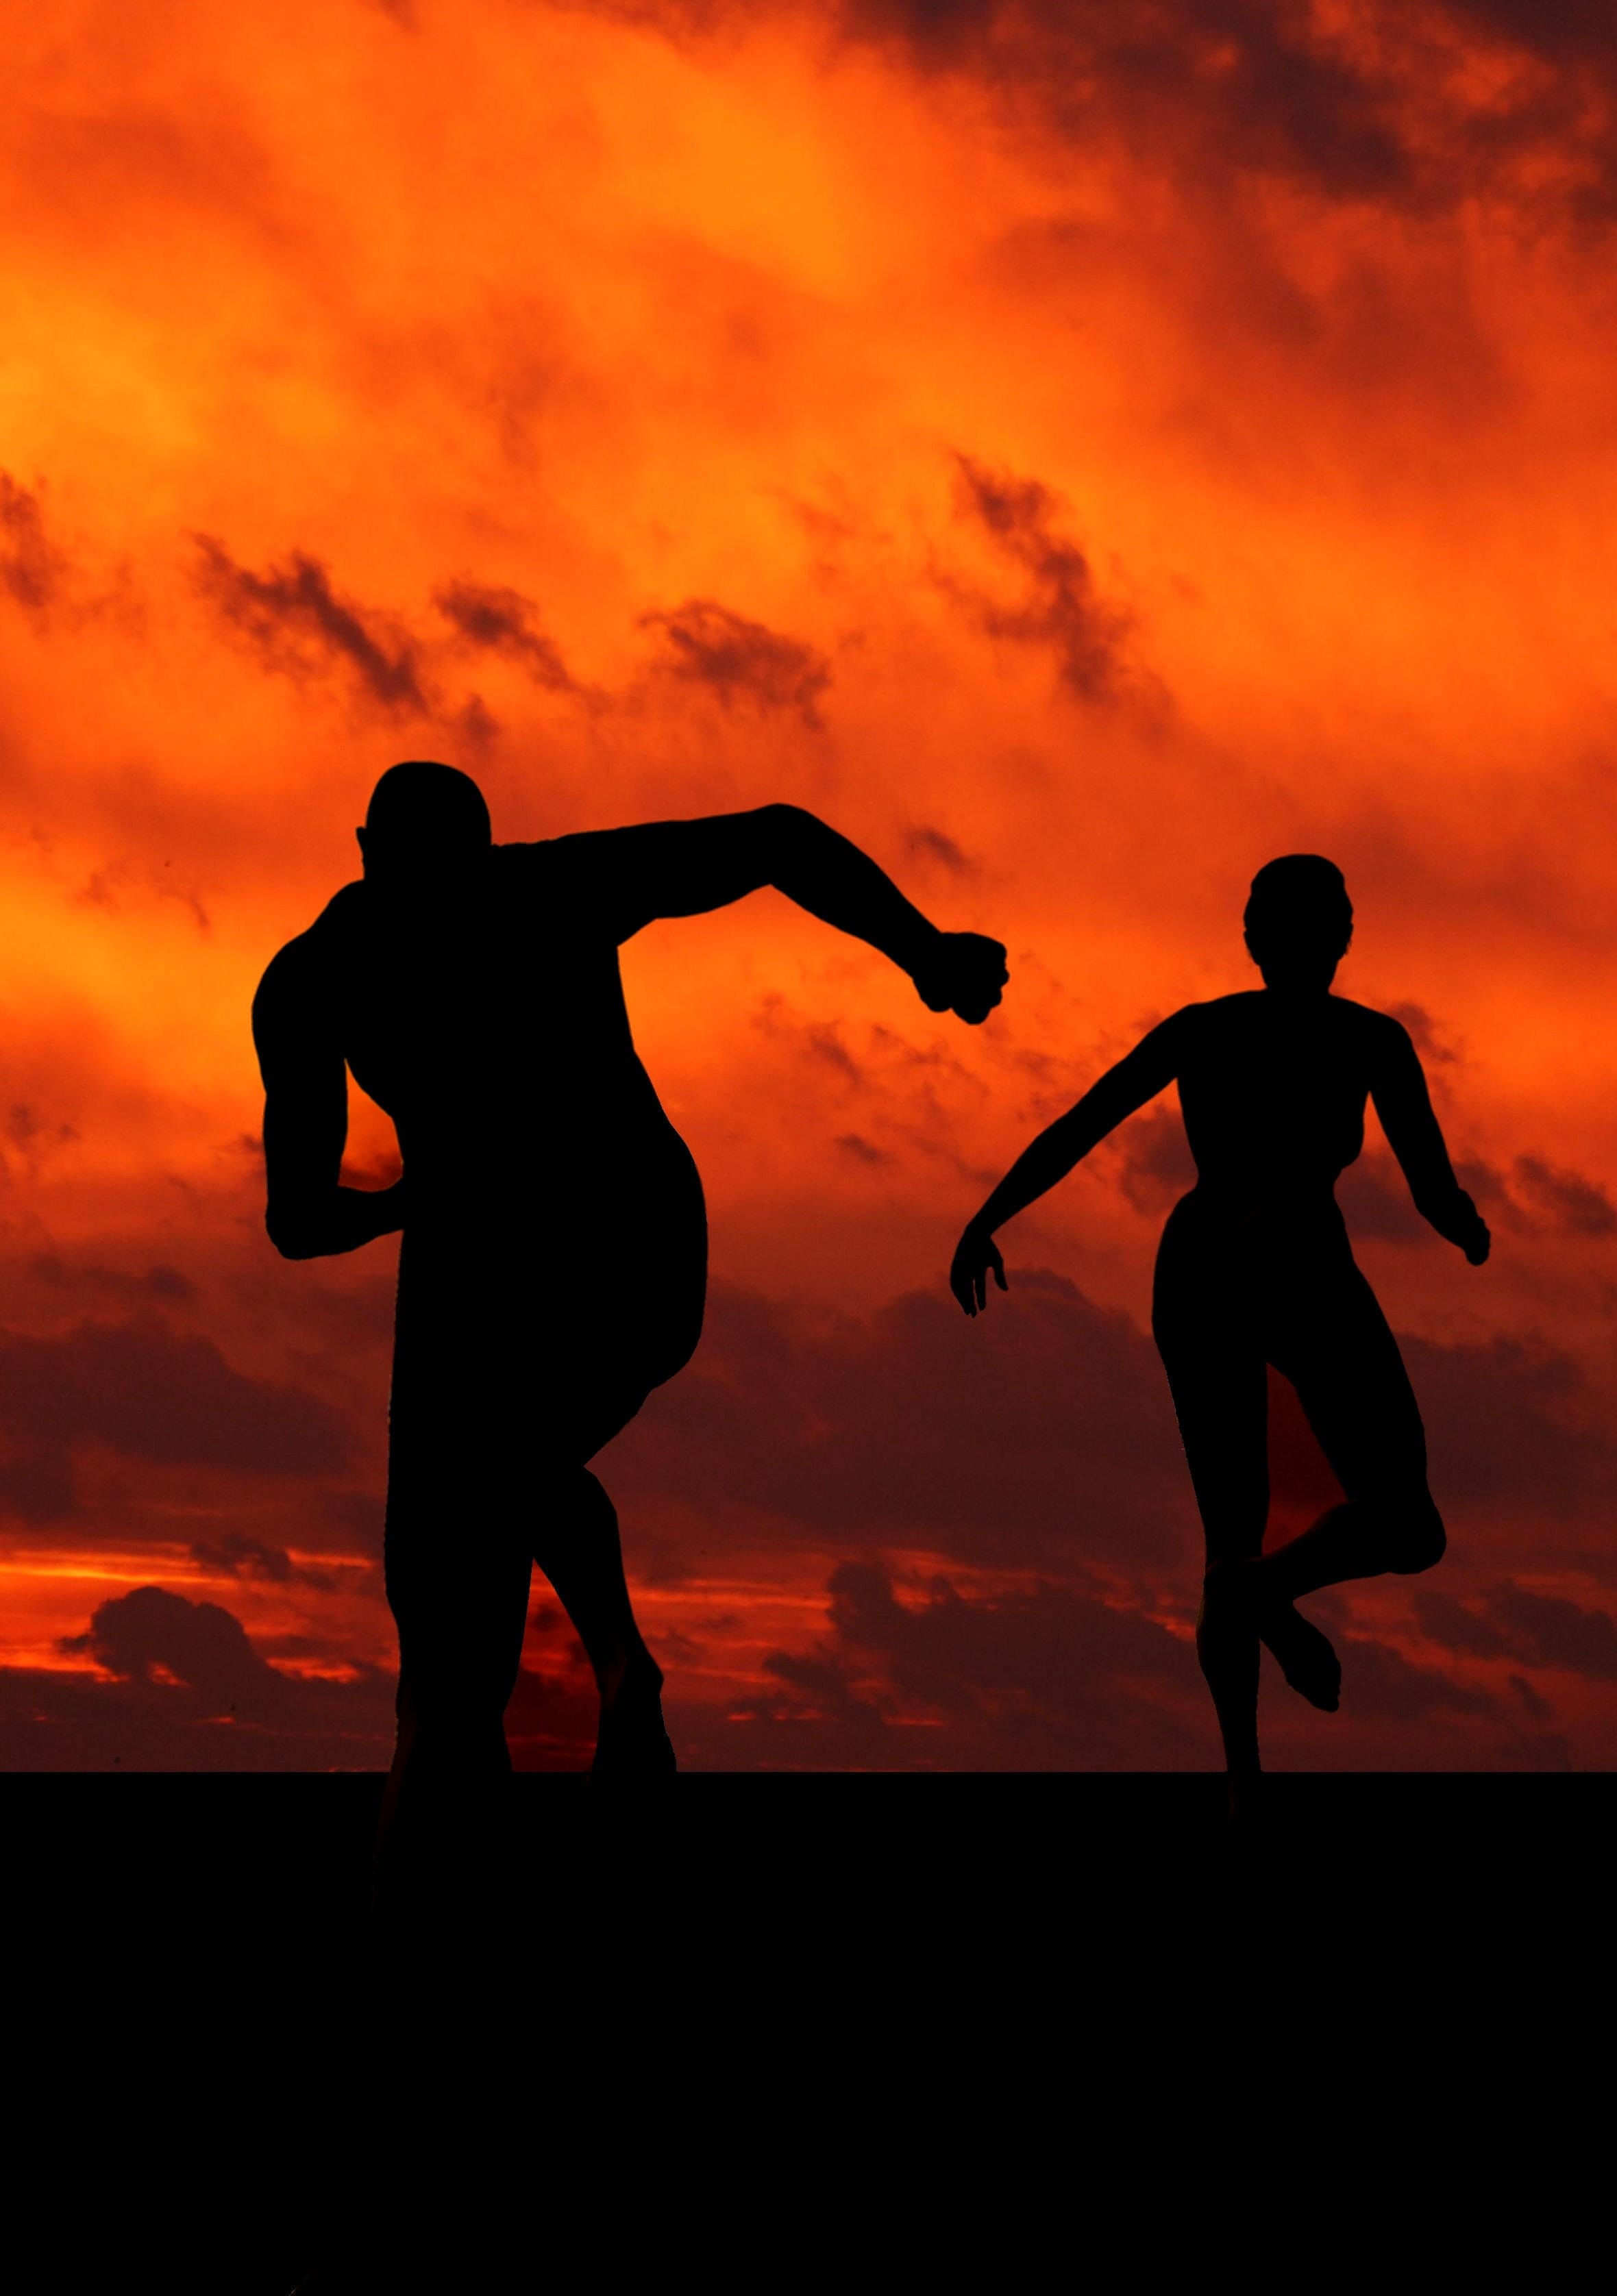
\includegraphics[width=\textwidth,height=12em]{images/sante-sport.jpg}

\end{center}

\hypertarget{jusquuxe0-quelle-fruxe9quence-dentrauxeenement-le-sport-est-il-vraiment-buxe9nuxe9fique-pour-la-santuxe9}{%
\subsection*{Jusqu'à quelle fréquence d'entraînement le sport est-il vraiment bénéfique pour la santé~?}\label{jusquuxe0-quelle-fruxe9quence-dentrauxeenement-le-sport-est-il-vraiment-buxe9nuxe9fique-pour-la-santuxe9}}
\addcontentsline{toc}{subsection}{Jusqu'à quelle fréquence d'entraînement le sport est-il vraiment bénéfique pour la santé~?}

La pratique sportive est généralement présentée comme une activité hautement bénéfique pour la santé physique et psychique. D'ailleurs, selon l'organisation mondiale de la santé, il est établi que la pratique régulière de sport favorise la prévention de nombreuses maladies notamment des maladies cardiaques, des accidents vasculaires cérébraux, du diabète, des cancers du sein et du côlon et contribue également à améliorer la santé mentale et la qualité de vie.

Cependant, l'excès de sport peut également avoir des effets néfastes et le surentrainement peut notamment favoriser les dépressions \footnote{Armstrong, L. E., \& VanHeest, J. L. (2002). The Unknown Mechanism of the Overtraining Syndrome. Sports Medicine, 32(3), 185-209} et peut également influencer de façon négative les performances cognitives des sportifs \footnote{Blain, B., Schmit, C., Aubry, A., Hausswirth, C., Meur, Y. L., \& Pessiglione, M. (2019).} \footnote{Neuro-computational Impact of Physical Training Overload on Economic Decision-Making. Current Biology, 29(19), 3289-3297.e4}.

Sans parler des accidents qui peuvent induire des blessures de différents niveaux de gravité dans certains sports, l'on peut se poser la question de savoir à partir de quand telle fréquence, telle intensité ou telle durée d'entraînement pourraient, au contraire, être néfastes pour l'humain. Que font les sportifs pour éviter les effets négatifs du surentrainement~?

\begin{signature}
\emph{Manuel Zenger}

\end{signature}

\hypertarget{le-sommeil}{%
\chapter{Le sommeil}\label{le-sommeil}}

\begin{center}
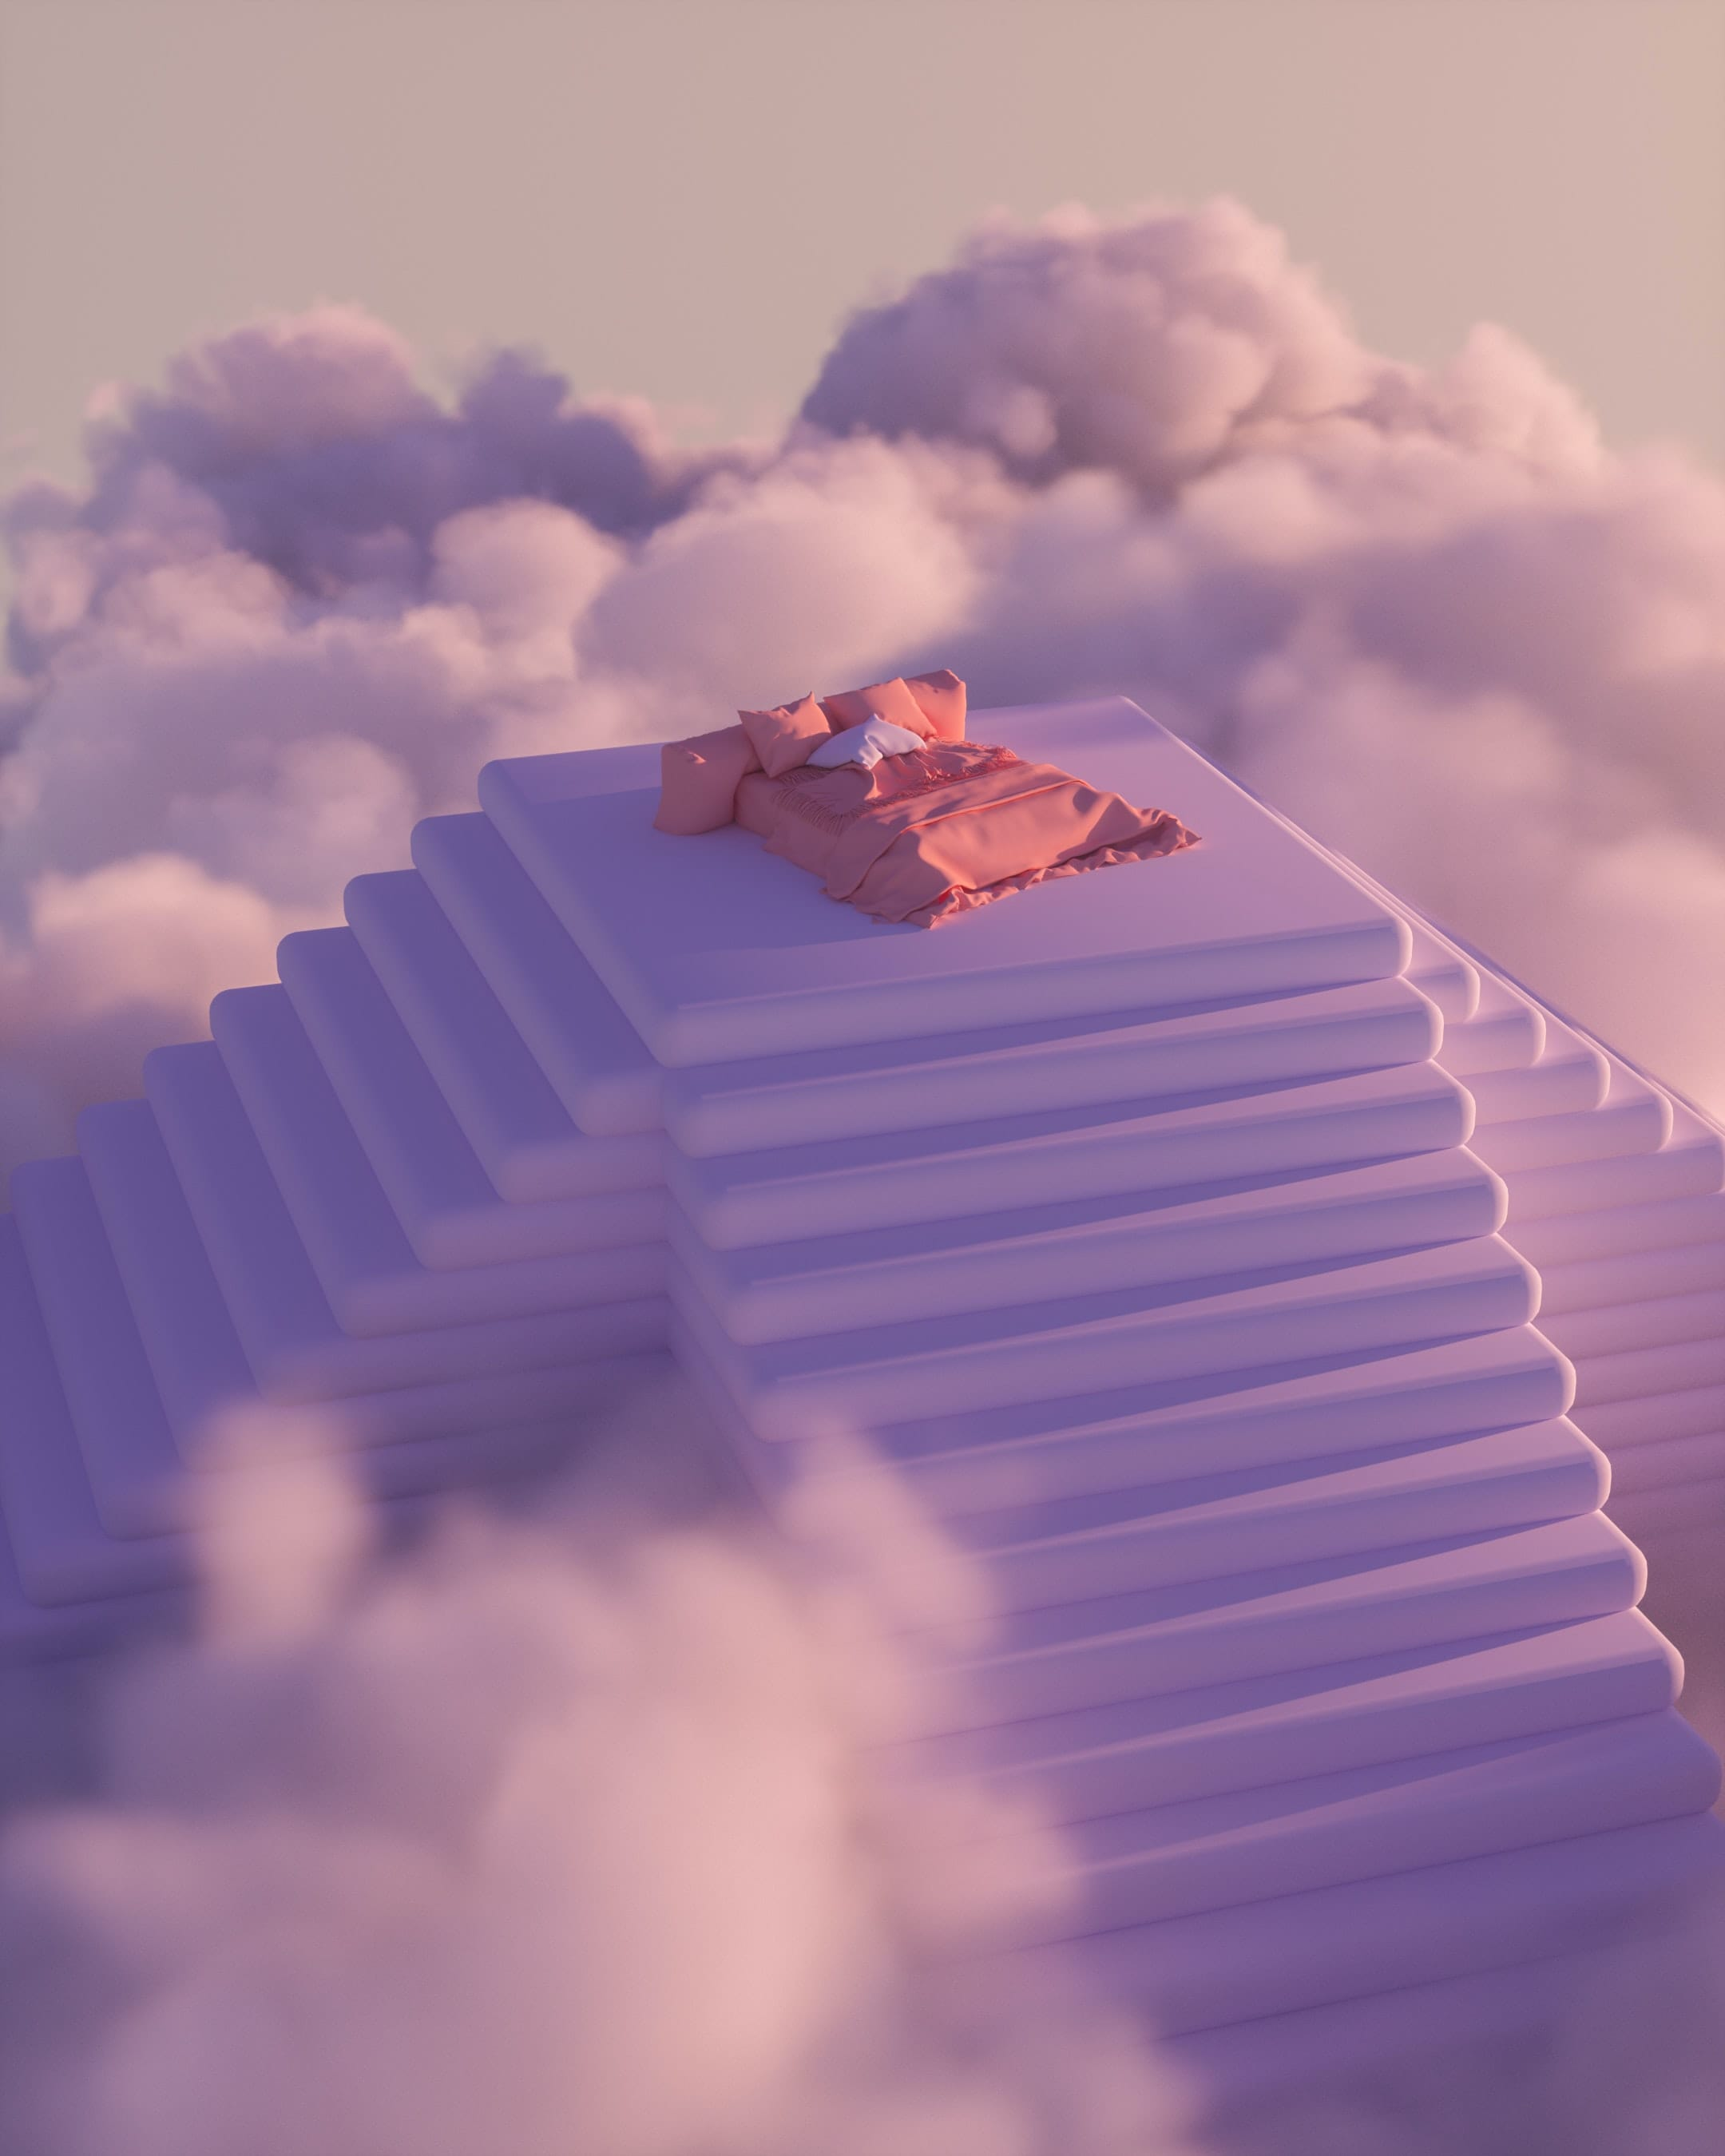
\includegraphics[width=\textwidth,height=12em]{images/sommeil.jpg}

\end{center}

\hypertarget{importance-et-influence-sur-la-santuxe9-physique-et-psychique}{%
\subsection*{Importance et influence sur la santé physique et psychique}\label{importance-et-influence-sur-la-santuxe9-physique-et-psychique}}
\addcontentsline{toc}{subsection}{Importance et influence sur la santé physique et psychique}

Si la durée du sommeil peut être très variable d'un individu à un autre, les besoins en sommeil sont également très différents selon l'âge de la personne~: pour un nouveau-né, 14-17 heures de sommeil sont recommandées par jour, pour un enfant de 1 an, 11 à 14 heures, pour un adolescent, 8 à 10 heures, pour un adulte, 7 à 9 heures par jour et pour une personne âgée, 7 à 8 heures (indications de la Fondation nationale américaine du sommeil (National Sleep Foundation)). La réalité individuelle du sommeil pour une personne peut toutefois être très différente~; les nombreuses activités, les situations stressantes ou d'autres raisons poussent parfois les individus à réduire leurs temps de sommeil. On peut s'interroger quant aux potentielles conséquences négatives sur la santé physique et/ou psychique qui surviennent lors d'un manque de sommeil.

Sans aller jusqu'au record d'absence de sommeil de Randy Gardner, étudiant américain, qui n'a pas dormis durant 11 jours et 25 minutes, des études indiquent que le manque de sommeil chronique est associé à des effets néfastes sur la santé, notamment la prise de poids et l'obésité, le diabète, l'hypertension, les maladies cardiaques et les accidents vasculaires cérébraux, la dépression et un risque accru de décès \footnote{Watson et al.~(2015). Recommended Amount of Sleep for a Healthy Adult: A Joint Consensus Statement of the American Academy of Sleep Medicine and Sleep Research Society. Journal of Clinical Sleep Medicine\,: JCSM\,: Official Publication of the American Academy of Sleep Medicine, 38.}.

Cette thématique pourrait être abordée de différentes manières lors d'un travail de maturité.

\begin{signature}
\emph{Manuel Zenger}

\end{signature}

\hypertarget{des-analyses-chimiques-avec-mon-tuxe9luxe9phone-portable}{%
\chapter{\texorpdfstring{Des analyses chimiques \linebreak avec mon téléphone portable}{Des analyses chimiques avec mon téléphone portable}}\label{des-analyses-chimiques-avec-mon-tuxe9luxe9phone-portable}}

\begin{center}
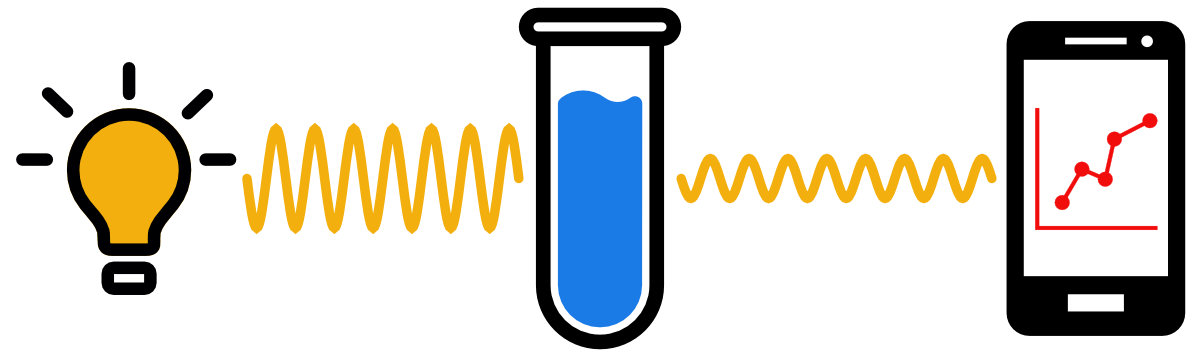
\includegraphics[width=\textwidth,height=12em]{images/analyses-chimiques-telephone-portable.jpg}

\end{center}

Les smartphones font partie intégrante de notre vie quotidienne, mais nous accordons peu d'attention à l'utilisation de leurs capteurs pour la collecte et l'analyse de données. En effet, ces appareils intègrent généralement un capteur d'image, un microphone, un accéléromètre, un gyroscope, un capteur de pression atmosphérique, une boussole numérique et bien d'autres instruments encore qui peuvent être extrêmement utiles dans un laboratoire de chimie.

Alors, pourquoi s'en priver et ne pas utiliser ces puissants appareils qui tiennent dans le creux de notre main pour résoudre des problèmes du laboratoire ?

La colorimétrie est une méthode d'analyse qui relie la variation de la couleur d'une solution à la concentration d'un soluté. Un colorimètre est un appareil coûteux et très utilisé en chimie et en biologie pour, par exemple, l'analyse du sang ou de l'eau, des nutriments du sol et des denrées alimentaires, la détermination des vitesses de réaction ou l'étude de la croissance de cultures bactériennes.

Ce thème de travail de maturité vous propose de concevoir et développer un dispositif d'analyse chimique permettant de transformer simplement n'importe quel téléphone portable en un colorimètre fiable.

\begin{signature}
\emph{Michele Rizzello}

\end{signature}

\hypertarget{chimie-et-photographie}{%
\chapter{Chimie et photographie}\label{chimie-et-photographie}}

\begin{center}
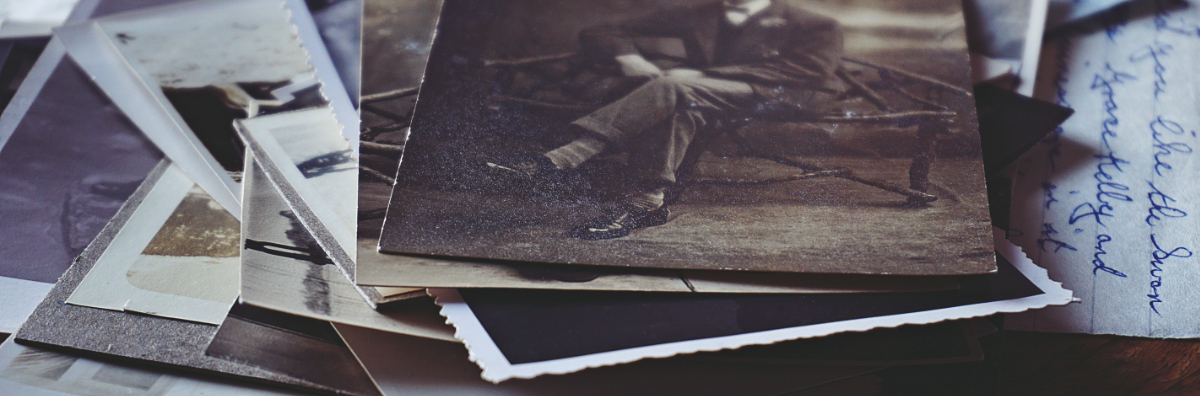
\includegraphics[width=1\textwidth,height=\textheight]{images/chimie-et-photographie.jpg}

\end{center}

\vspace{\stretch{1}}

\hypertarget{un-sujet-pour-les-uxe9luxe8ves-photosensibles}{%
\subsection*{Un sujet pour les élèves photosensibles}\label{un-sujet-pour-les-uxe9luxe8ves-photosensibles}}
\addcontentsline{toc}{subsection}{Un sujet pour les élèves photosensibles}

Les nouvelles technologies permettent d'avoir en permanence sur soi un appareil photo. Lorsque nous prenons une photo, nous sommes aujourd'hui habitués à une récompense instantanée~: on regarde un écran numérique, on clique sur un bouton et l'on obtient une image parfaite. Mais il n'en a pas toujours été ainsi~\ldots{}

Ce thème de travail de maturité est une exploration de la chimie de la photographie par l'expérience pratique. Vous élargirez vos connaissances de la technique photographique et de la fabrication de tirages, tout en appliquant la chimie que vous apprenez en cours.

L'objectif du projet est de recréer un ou plusieurs procédés chimiques traditionnellement utilisés pour le développement avec des produits domestiques de substitution et être capable d'expliquer, grâce à leurs propriétés chimiques, pourquoi ces substitutions fonctionnent. Le produit fini sera un procédé que n'importe qui pourrait créer, sans accéder à des fournitures photographiques coûteuses.

\begin{signature}
\emph{Michele Rizzello}

\end{signature}

\hypertarget{leau-chaude-guxe8le-t-elle-plus-vite-que-leau-froide}{%
\chapter{\texorpdfstring{L'eau chaude gèle-t-elle \linebreak plus vite que l'eau froide~?}{L'eau chaude gèle-t-elle plus vite que l'eau froide~?}}\label{leau-chaude-guxe8le-t-elle-plus-vite-que-leau-froide}}

\begin{center}
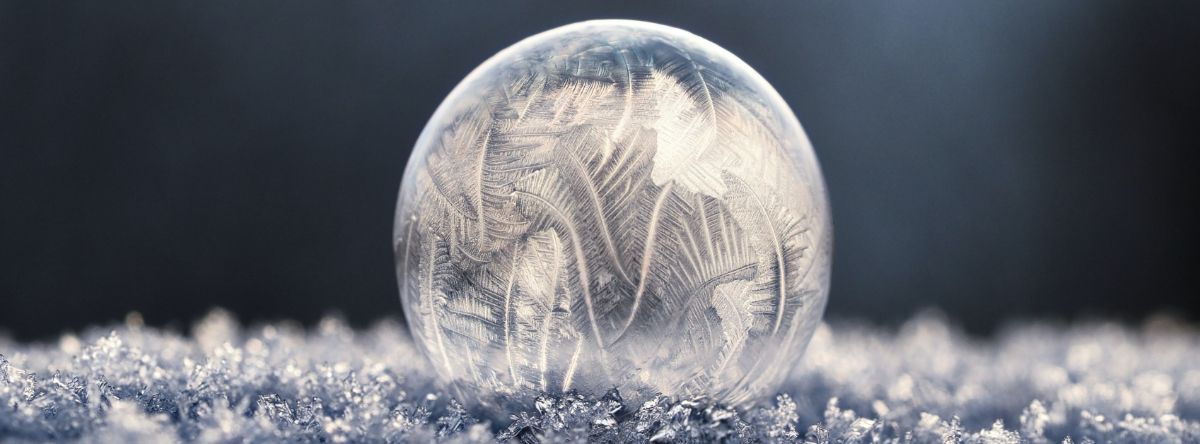
\includegraphics[width=1\textwidth,height=\textheight]{images/eau-chaude.jpg}

\end{center}

On pourrait dire que c'est une des expériences les plus simples qui soient. Prenez deux récipients, un rempli d'eau chaude et l'autre rempli d'eau froide. Placez-les dans un congélateur et notez laquelle gèle en premier. Le bon sens suggère que l'eau froide gèlera en premier. Cependant, depuis l'Antiquité, on observe que, sous certaines conditions, l'eau chaude peut refroidir plus vite.

Ce phénomène a été porté à l'attention du public en 1963 par un étudiant tanzanien de 17 ans, Erasto Mpemba. Accidentellement, il a découvert que la glace qu'il avait fabriquée en congelant un mélange chaud avait gelé avant celle de ses camarades, réalisée avec des mélanges froids. Quand il raconta à son professeur ce qu'il avait observé, le professeur lui dit qu'il avait dû se tromper. Personne ne l'a cru.

Mpemba n'a pas baissé les bras et a présenté ses observations à un professeur d'université qui visitait son école. Le professeur a tenté l'expérience, il l'a confirmée et ils ont ensuite coécrit un article à ce sujet qui fut en 1969. Au fil des ans, de nombreuses personnes ont essayé de reproduire cette expérience, certaines ont réussi et d'autres ont échoué. Aujourd'hui encore, il existe une controverse sur les bases théoriques et sur les paramètres nécessaires pour reproduire cet effet.

Le but de ce travail de maturité sera de concevoir et tester un dispositif technique permettant d'observer le phénomène et de tenter de fournir une explication à cet effet, connu aujourd'hui sous le nom d'effet Mpemba.

\begin{signature}
\emph{Michele Rizzello}

\end{signature}

\hypertarget{les-additifs-en-cosmuxe9tiques}{%
\chapter{Les additifs en cosmétiques}\label{les-additifs-en-cosmuxe9tiques}}

\begin{center}
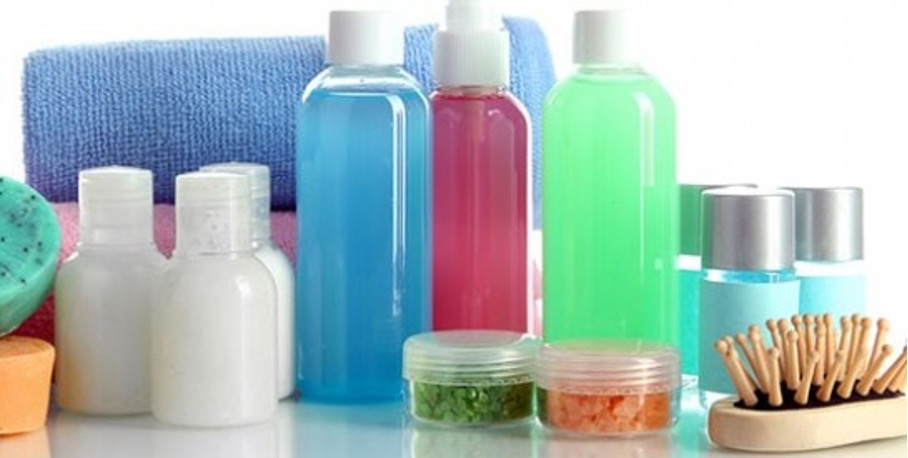
\includegraphics[width=\textwidth,height=12em]{images/les-additifs-en-cosmetiques.jpg}

\end{center}

Tous les jours, dès notre réveil, nous utilisons de nombreux cosmétiques. On se dirige vers la salle de bain pour prendre une douche~; le shampoing est appliqué sur nos cheveux et notre corps est délicatement lavé avec un produit approprié. Une fois séché, un coup de rasoir puis un peu de déodorant, de crème hydratante et pourquoi pas de maquillage seront encore ajoutés. Après le petit déjeuner, nos dents sont brossées avec du dentifrice, nos mains sont lavées au savon. Et avant de s'en aller, encore un pschitt de parfum, la journée ne fait que commencer.

Ces produits cosmétiques sont composés de différents ingrédients qui peuvent être d'origine animale, végétale, minérale ou, dans la plupart des cas, être créés artificiellement. Ils contiennent également un certain nombre d'additifs, naturels ou de synthèse, qui leur permettent, entre autres, d'être conservés plus longtemps, de les colorer, de les parfumer, de les humidifier ou d'améliorer leur texture.

\clearpage

Le but de ce travail de maturité est de s'intéresser à la composition des cosmétiques ou à l'un d'entre eux en particulier. Cette recherche pourra être abordée de différentes manières en fonction de vos intérêts et vous pourrez, par exemple~:

\begin{itemize}
\tightlist
\item
  Analyser les différents additifs présents dans les cosmétiques
\item
  Étudier les parfums, leur histoire ainsi que leur création
\item
  Analyser la dangerosité des additifs et trouver des alternatives
\item
  Étudier les colorants, leur synthèse ainsi que leur utilisation
\item
  Étudier la chimie du savon, son histoire, sa fabrication et ses propriétés
\item
  Il sera également possible de réaliser en laboratoire, dans la mesure du possible, le produit ou l'additif étudié.
\end{itemize}

\begin{signature}
\emph{Mélanie Tschirren}

\end{signature}

\hypertarget{fluorescence-et-phosphorescence}{%
\chapter{Fluorescence et phosphorescence}\label{fluorescence-et-phosphorescence}}

\begin{center}
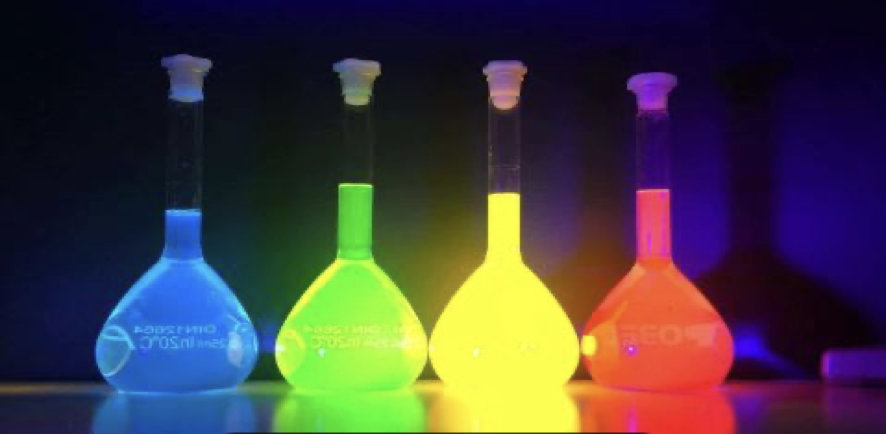
\includegraphics[width=\textwidth,height=12em]{images/fluorescence-et-phosphorescence.jpg}

\end{center}

\vspace{\stretch{1}}

La luminescence est un terme générique qui englobe la fluorescence et phosphorescence. Il s'agit de la transformation par la matière d'énergie en émission lumineuse. Ce phénomène est connu depuis des siècles~: n'avons-nous pas de tout temps été émerveillés par un ballet de lucioles par une belle nuit d'été~?

Ces dernières dizaines d'années, l'utilisation de ce phénomène dans des applications industrielles et de la vie de tous les jours a pris une ampleur considérable, si bien que le contrôle des sources d'approvisionnement et des techniques de productions des matériaux luminescents est devenu un enjeu stratégique majeur, au vu du l'avantage concurrentiel que procure leur maîtrise.

Nous avons tous en tête les feutres fluorescents d'une marque bien connue qui nous servent à surligner des éléments importants d'un texte, mais l'application des matériaux luminescents est bien plus large. Elle va des écrans de haute qualité, aux sources de lumières telles que les ampoules LED ou aux bandes de sécurité nous guidant lors d'évacuation des immeubles en cas d'incendie.

\clearpage

Le thème de ce travail de maturité est d'étudier comment le phénomène de fluorescence ou phosphorescence est utilisé et fonctionne dans une application industrielle donnée ; il s'agira également de traiter les éléments stratégiques, économiques et écologiques qui se cachent derrière la maîtrise de ces matériaux et de leur usage.

\begin{signature}
\emph{Claude-Alain Despland}

\end{signature}

\hypertarget{cest-pas-sorcier}{%
\chapter{C'est pas sorcier}\label{cest-pas-sorcier}}

\begin{center}

\includegraphics[width=\textwidth,height=12em]{images/cest-pas-sorcier.jpg}

\end{center}

\vspace{\stretch{1}}

\hypertarget{mettre-en-scuxe8ne-un-sujet-scientifique-uxe0-la-maniuxe8re-de-la-cuxe9luxe8bre-uxe9mission-de-france-3-avec-les-personnages-iconiques-de-fred-et-jamy.}{%
\subsection*{Mettre en scène un sujet scientifique à la manière de la célèbre émission de France 3 avec les personnages iconiques de Fred et Jamy.}\label{mettre-en-scuxe8ne-un-sujet-scientifique-uxe0-la-maniuxe8re-de-la-cuxe9luxe8bre-uxe9mission-de-france-3-avec-les-personnages-iconiques-de-fred-et-jamy.}}
\addcontentsline{toc}{subsection}{Mettre en scène un sujet scientifique à la manière de la célèbre émission de France 3 avec les personnages iconiques de Fred et Jamy.}

\vspace{\stretch{1}}

La première étape consistera à trouver un sujet scientifique qui vous intrigue et qui n'a pas été traité dans les épisodes de \emph{C'est pas sorcier}.

Vous aurez ensuite l'opportunité de rédiger un scénario, devenir acteur et animateur, monter des expériences et des démonstrations en laboratoire ou sur scène, interviewer des experts, réaliser un reportage et finalement un montage vidéo de 20 minutes environ, pour explorer et expliquer le sujet que vous avez choisi.

Le but final de ce travail de maturité sera la réalisation d'un véritable documentaire audiovisuel qui traitera de manière scientifique le sujet abordé. Chaque projet sera basé sur une solide documentation qui permettra ensuite la réalisation d'un scénario, de décors, de maquettes.

\clearpage

En devenant chef de votre projet, vous ferez appel à toutes les ressources possibles. Pour certaines compétences techniques (prise de vue, montage vidéo), il sera nécessaire de rechercher des personnes qualifiées dans votre entourage.

Ce travail de maturité se fait obligatoirement par groupes de deux.

\begin{signature}
\emph{Jonathan Monteverde}\\
\emph{Nicolas Cusnir}\\
\emph{Gwenola Tabin}

\end{signature}

\hypertarget{changement-climatique-et-sociuxe9tuxe9s}{%
\chapter{Changement climatique et sociétés}\label{changement-climatique-et-sociuxe9tuxe9s}}

\begin{center}
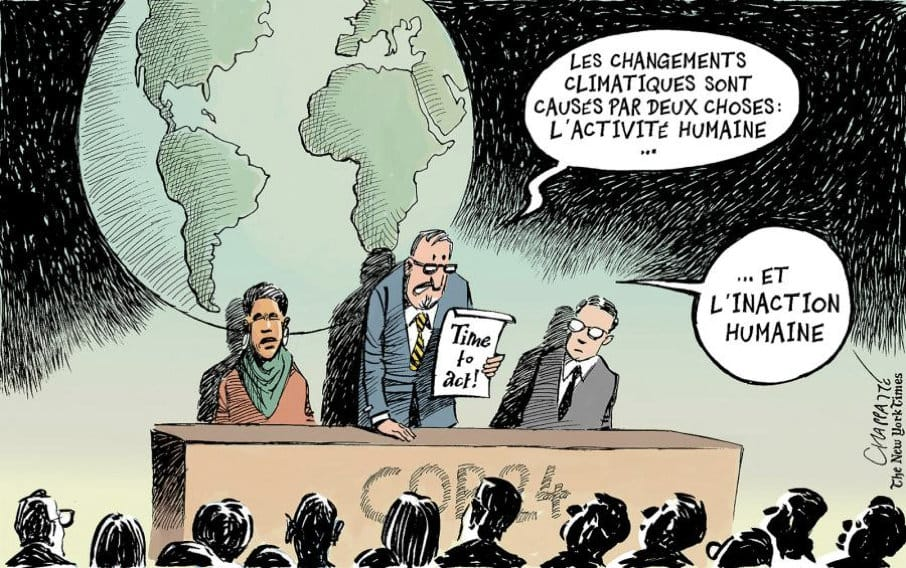
\includegraphics[width=\textwidth,height=18em]{images/changement-climatique-et-societes.jpg}\\
\footnote{© Chappatte dans The New York Times, 2018}

\end{center}

\vspace{\stretch{1}}

\emph{``~Le climat change, peut-être que nous devrions faire de même\ldots~''.}

\vspace{\stretch{1}}

Un étroit lien existe entre le changement climatique et les sociétés humaines à travers le globe. D'un point de vue géographique, cette thématique doit vous permettre de vous intéresser à un phénomène propre aux changements climatiques tout en analysant les causes, les effets, les enjeux pour une ou plusieurs sociétés ainsi que les perspectives concrètes pour limiter les impacts du changement climatique. Que ce soit l'exploitation de ressources, le réchauffement climatique, l'augmentation des niveaux des océans, la désertification des territoires ou encore la destruction de la biodiversité, il s'agira pour vous de lier et de comprendre les influences réciproques qu'il peut y avoir entre un phénomène climatique et les impacts pour une société, pour un territoire ou pour une population.

\clearpage

Quel que soit le sujet de votre choix, il s'agira pour vous d'identifier une problématique et de l'étudier dans une perspective durabiliste. Il s'agira également de comprendre et d'interpréter les différentes interactions qui prennent place entre cet environnement naturel et les sociétés humaines qui exploitent, subissent ou modifient leur espace de vie.

Ce TM est recommandé pour des groupes de 2 élèves.

\begin{signature}
\emph{Cyril Kull}

\end{signature}

\hypertarget{luxe9quilibre-entre-la-vie-professionnelle-et-la-vie-privuxe9-des-jeunes-adultes}{%
\chapter{\texorpdfstring{L'équilibre entre la vie professionnelle \linebreak et la vie privé des jeunes adultes}{L'équilibre entre la vie professionnelle et la vie privé des jeunes adultes}}\label{luxe9quilibre-entre-la-vie-professionnelle-et-la-vie-privuxe9-des-jeunes-adultes}}

\begin{center}
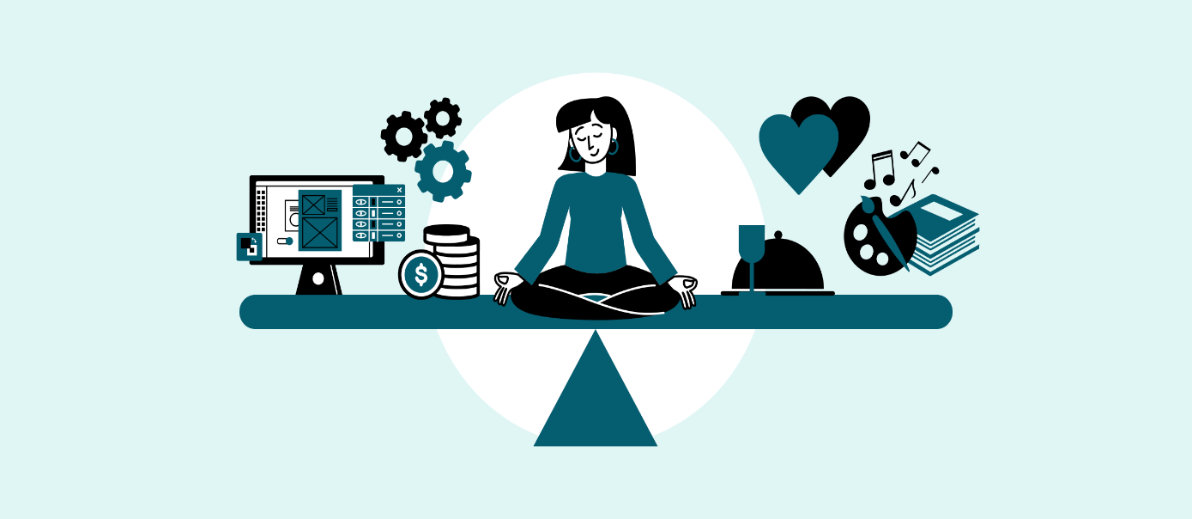
\includegraphics[width=\textwidth,height=12em]{images/equilibre-vie-professionnelle-prive-jeunes-adultes.jpg}

\end{center}

Est-ce que les jeunes diplômés veulent plus de flexibilité dans leur travail ? Travailler moins pour travailler mieux ?

Les jeunes diplômés aspirent à un meilleur équilibre entre vie professionnelle et vie privée et sont de plus en plus nombreux à vouloir travailler à temps partiel ; les jeunes demandent aussi plus d'autonomie et d'indépendance dans leur travail.

La flexibilité est devenue une aspiration quasiment universelle, accélérée par la pandémie de Covid.

Ce travail de maturité devra déboucher sur des recherches concrètes (un sondage et/ou un interview par exemple) pour comprendre

Une tendance que confirme Darryl Lüthi, coach chez ``\href{mailto:Jeunes@work}{\nolinkurl{Jeunes@work}}'' (coaching gratuit et passerelle vers le premier emploi, \href{mailto:Jeunes@Work}{\nolinkurl{Jeunes@Work}} prépare efficacement les jeunes diplômés à intégrer le marché du travail et permet aux entreprises de recruter les talents de demain) :``Il y a eu un changement de paradigme ces cinq dernières années. Avant, l'emploi occupait une place centrale dans la vie d'un candidat, et la vie privée se construisait autour du travail. Aujourd'hui, l'emploi ne représente plus une fin en soi''.

Ce travail de maturité devra déboucher sur des recherches concrètes (un sondage et/ou un interview par exemple) pour comprendre les attentes des jeunes dans leur future vie professionnelle et pour découvrir comment les jeunes adultes perçoivent aujourd'hui l'équilibre entre le travail et la vie privé.

Ce TM est recommandé pour des groupes de 2 élèves.

\begin{signature}
\emph{Mirko Maternini}

\end{signature}

\hypertarget{le-droit-dans-lunivers-dharry-potter}{%
\chapter{Le droit dans l'univers d'Harry Potter}\label{le-droit-dans-lunivers-dharry-potter}}

La saga de J.K. Rowling est un phénomène mondial, de portée intergénérationnelle. Les contemporains aux personnages de l'époque, relate aujourd'hui les aventures d'Harry, Ron et Hermione à ses propres enfants. Cet univers magique dépeint une société fantasmagorique s'organisant selon des règles mystérieuses. Bien qu'au premier abord sa structure paraisse très éloignée du nôtre, en laissant de côté baguettes magiques et balais volants pour s'intéresser à l'essence même du fonctionnement de ces sorciers, ne pourrions-nous pas trouver des similitudes~avec notre état ?

\begin{center}
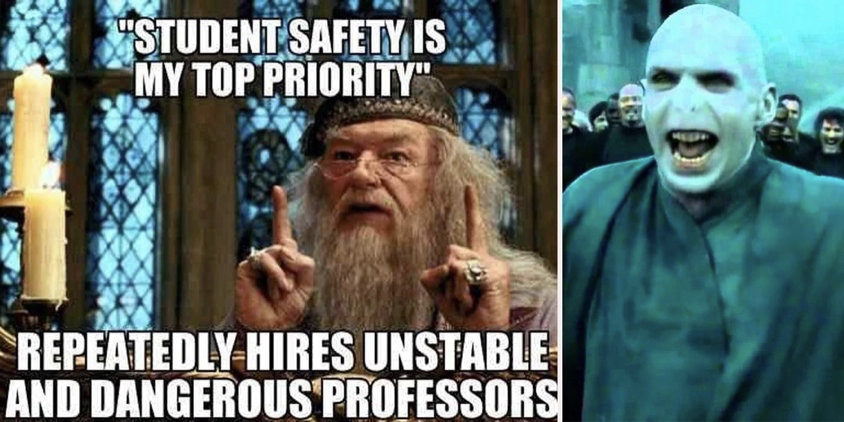
\includegraphics[width=\textwidth,height=12em]{images/le-droit-dans-lunivers-dharry-potter-1.jpg}

\end{center}

Que ce soit la Constitution avec notamment l'organisation du ministère de la magie, le droit Pénal appliqué à la prison d'Azkaban, le droit du Sport lors des compétitions de Quidditch, le statut des créatures magiques, de nombreux parallèles sont à faire. L'analyse peut être poussée sur une réflexion sociétale et éthique du droit, en prenant également compte les différences, lacunes et dérives de notre système juridique actuel. Pensons par exemple à la notion d'état d'urgence appliquée lors du Covid ou aux Droits de l'Homme mis à mal lors de l'organisation de la coupe de monde de football au Qatar.

\begin{center}
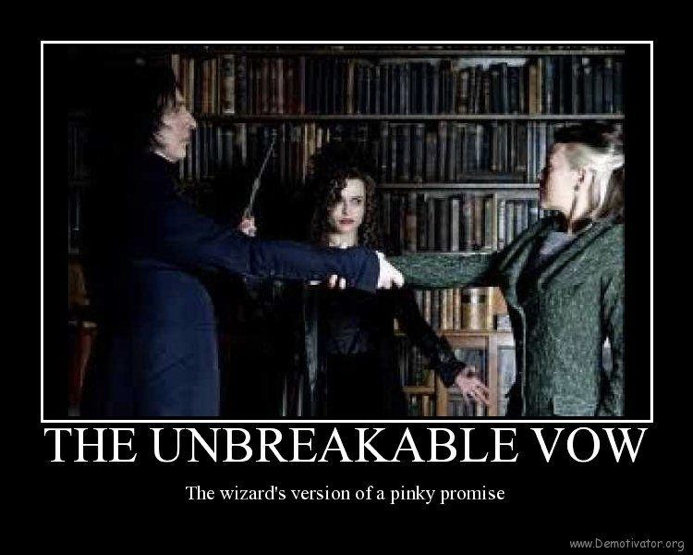
\includegraphics[width=\textwidth,height=12em]{images/le-droit-dans-lunivers-dharry-potter-2.jpg}

\end{center}

Dans ce travail vous aurez l'opportunité d'approfondir une problématique d'un domaine du droit qui vous intéresse. Vous pourrez ensuite laisser parler votre créativité en extrapolant ces règles dans le monde magique d'Harry Potter. Préparez-vous à entamer un voyage enchanteur et laissez-vous séduire par la logique propre au monde de la sorcellerie\ldots{}

\begin{signature}
\emph{Morgane Fibicher}

\end{signature}

\hypertarget{philosophie-de-lart-la-beautuxe9-et-la-vuxe9rituxe9}{%
\chapter{Philosophie de l'art : La beauté et la vérité}\label{philosophie-de-lart-la-beautuxe9-et-la-vuxe9rituxe9}}

Que la beauté soit une affaire de goût, qu'elle soit subjective, qu'elle soit relative et propre à chacun, c'est ce qui semble aller de soi. Mais que dire du chef-d'œuvre qui prétend à l'universalité~? Que dire du jugement esthétique qui s'offusque lorsqu'on le contrarie~? Une fleur est belle, un paysage est beau, un visage est beau~: n'est-ce pas à dire que la beauté se situe dans les choses~? Qu'elle est objective~? Mais alors, comment se dévoile-t-elle~? Est-ce par une modification du regard chez l'observateur, par un travail de l'artiste sur la chose qu'il façonne, ou par l'éclat à peine aperçu d'un objet qui suggère qu'il dissimule un secret~? Pouvons-nous nous contenter de regarder une œuvre d'art ou devons-nous la contempler~? Et l'artiste, dès lors, est-il un créateur ou un voyant~? Il n'est pas rare d'ailleurs que nous ressentions un sentiment d'authenticité face à une œuvre d'art --~comme si là, en face de nous, c'était la vérité qui s'exprimait. Ce sentiment équivaut-il à une émotion~? Une réaction à une réalité qui donne des frissons~? Mais si c'est la vérité qui se manifeste dans une œuvre d'art~-- est-ce à dire que la science ne possède pas le monopole du savoir~? Que la science et l'art seraient des disciplines opposées, voire incompatibles~? Rien n'est moins sûr. Mais nous entendons que l'art a pour fonction d'imiter la nature, alors que la science l'explique et la décrit. Ne serait-ce pas que l'art a pour fonction d'embellir la nature~? Mais que dire alors des œuvres sublimes qui accentuent la laideur physique et la dégradation morale de ses sujets~? Que dire des caricatures, par exemple, desquelles se dégagent indiscutablement une modalité du beau et du vrai~? Accentuer les traits, déformer les corps, exagérer les expressions~: n'est-ce pas mentir~? Que dire des dissonances musicales qui semblent rompre un ordre harmonique qui est si doux à nos oreilles~? Représenter iconographiquement des êtres célestes et divins, n'est-ce pas profaner des entités qui dépassent la condition de l'homme~? Très rapidement s'est posée la question de savoir comment exprimer une idée artistique.

Nous pourrions en outre nous demander si l'expression artistique est une activité proprement humaine. Ne voyons-nous pas des araignées construire des édifices symétriques, dont la régularité surpassent parfois nos efforts architecturaux~? N'observons-nous pas dans la nature de nombreux actes de séduction animalière qui laissent entendre que les animaux possèdent aussi une sensibilité esthétique ? Peut-être que l'harmonie de la nature nous a conféré des normes artistiques dont il est difficile de nous défaire.

Tel serait un échantillon des questions qui peuvent être soulevées dans ce Travail de Maturité. Avec l'aide de textes appartenant à la tradition philosophique, mais aussi à la littérature, à la poésie, et aux artistes eux-mêmes --~qui ont souvent écrit sur leur pratique~--, nous nous interrogerons sur l'attrait qu'exerce sur nous le pouvoir des créations artistiques. Qu'il s'agisse du plaisir indescriptible qu'éveille la jouissance artistique, du moment de suspens que provoque en nous l'expérience esthétique elle-même, du basculement par lequel nous nous perdons dans un tableau, dans une sculpture, dans un morceau de musique, ou dans un film, du sérieux ou du jeu avec lesquels nous nous approchons d'une œuvre d'art, du milieu dans lequel l'œuvre d'art doit ou peut être appréhendée (théâtre, musée, chez soi, nature), de la modification que lui fait subir les impératifs de consommation, nous nous attacherons à montrer que la création artistique possède une place fondamentale dans notre rapport au monde.

Ce Travail de Maturité est ouvert à tous et n'exige aucun prérequis. Il demande simplement un intérêt pour la question artistique, une envie de penser, et une dose de curiosité.

\begin{signature}
\emph{Jeremy Filthuth et Esma Puric}

\end{signature}

\hypertarget{au-deluxe0-de-lhumain-transhumanisme-et-intelligence-artificielle-quelles-repruxe9sentations-et-quels-enjeux}{%
\chapter{\texorpdfstring{Au-delà de l'humain~: \linebreak transhumanisme et intelligence artificielle, quelles représentations et quels enjeux~?}{Au-delà de l'humain~: transhumanisme et intelligence artificielle, quelles représentations et quels enjeux~?}}\label{au-deluxe0-de-lhumain-transhumanisme-et-intelligence-artificielle-quelles-repruxe9sentations-et-quels-enjeux}}

\begin{center}
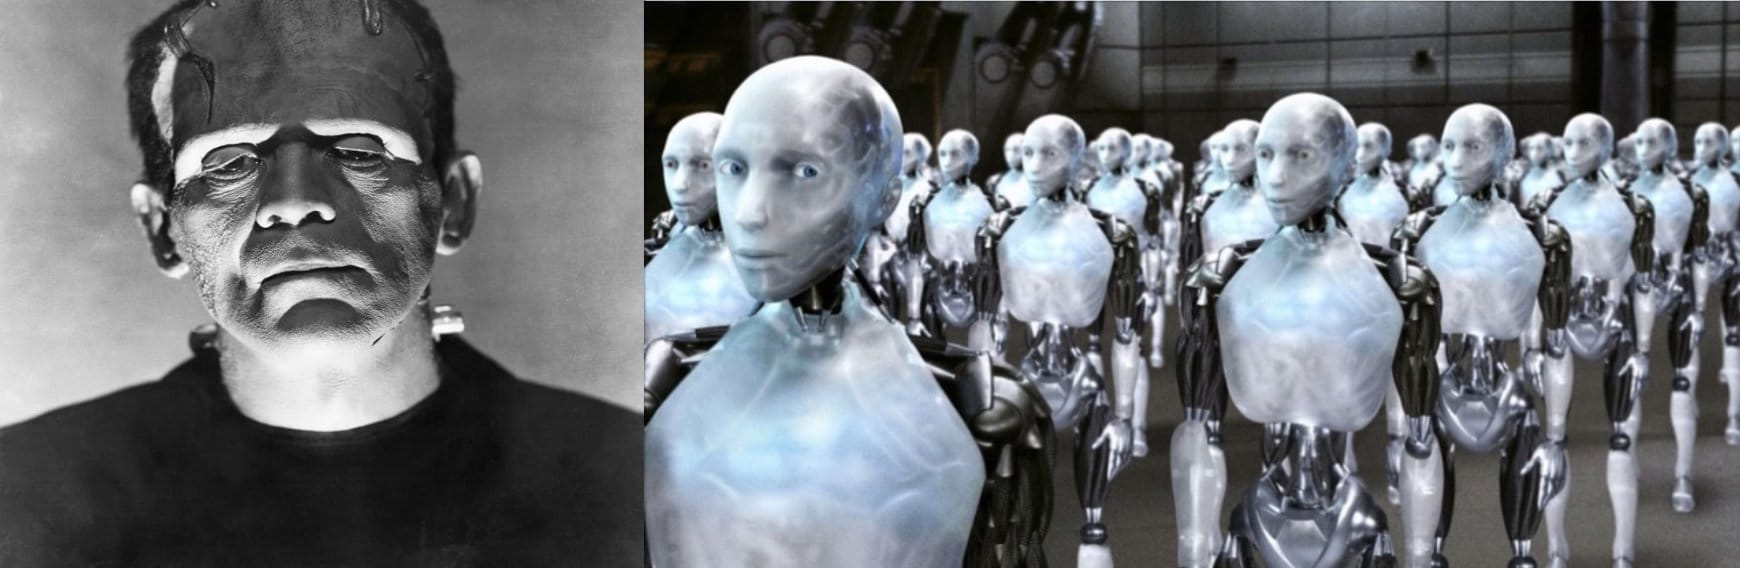
\includegraphics[width=\textwidth,height=12em]{images/au-dela-de-lhumain.jpg}\\
\footnote{Images~: La Créature, dans le film Frankenstein réalisé par James Whale (1931)~; Les robots dans I, Robot réalisé par Alex Proyas (2004).}

\end{center}

\vspace{\stretch{1}}

Le corps vieillit, la pensée demeure. Mais pourrait-elle nous survivre~? Pourrions-nous la déplacer sur un autre support~? Mais ce faisant, serions-nous alors toujours les mêmes~? Sur quoi repose la conscience~? Est-ce une entité totalement déconnectée du corps ou peut-on la recréer sur une base physique robotique ?
Améliorer le corps humain, supprimer son vieillissement et ainsi nier la mort, voilà ce que cherche le courant philosophique du transhumanisme. Science-fiction~? Abomination~? Progrès médicaux nécessaires~? Cette quête fait débat.

Ce travail de maturité questionnera les bénéfices de cette théorie ainsi que ses dérives potentielles. Les angles de réflexion pourront être philosophiques et éthiques mais également faire écho aux représentations littéraires et cinématographiques en analysant des œuvres telles que Frankenstein, Her, Ex machina, Transcendance, Matrix ou encore I, Robot.

\clearpage

Ce travail de maturité doit être réalisé en binôme et peut être rédigé en français ou en anglais.

\begin{signature}
\emph{Pauline Meylan et Swaha Somanadan}

\end{signature}

\hypertarget{le-jeu-viduxe9o-fiction-ou-ruxe9alituxe9}{%
\chapter{Le jeu vidéo : fiction ou réalité~?}\label{le-jeu-viduxe9o-fiction-ou-ruxe9alituxe9}}

\vspace{\stretch{1}}

\begin{center}
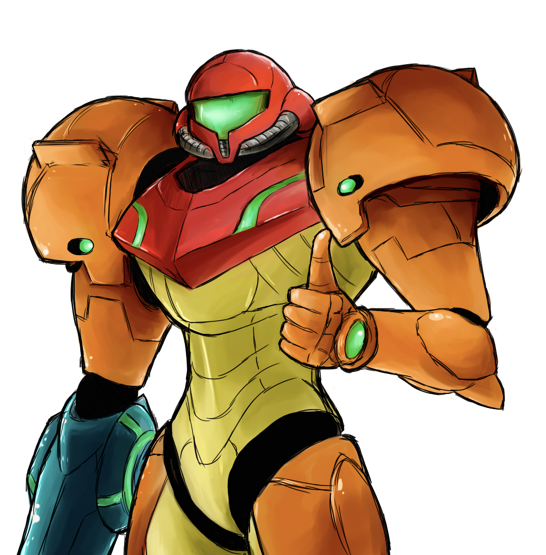
\includegraphics[width=\textwidth,height=12em]{images/le-jeu-video-fiction-ou-realite.jpg}

\end{center}

\vspace{\stretch{1}}

Depuis une dizaine d'années, la pratique du jeu vidéo s'est répandue à une large partie de la population. Bien que de nombreuses personnes aient accusé ce divertissement d'être à l'origine de violences ou de provoquer l'isolement des gameurs-euses, nous parlons actuellement du 10\textsuperscript{e} art pour nommer les jeux vidéo.

La stratégie de cette industrie ne repose pas uniquement sur le degré de divertissement qu'ils procurent, mais également sur leur impact visuel comme intellectuel. Ainsi a-t-on réalisé d'impressionnants progrès dans le développement réaliste des graphiques et dans la complexité de leur scénario.

Tout en laissant place à des produits originaux et conceptuels, les développeurs-ses tendent donc à mêler le réel à la fiction en ouvrant le champ à de nouvelles réflexions : comment représenter la société, le genre, la femme~? Comment simuler l'histoire, la gestion, les métiers~? Comment vous permettre à vous, gameurs-euses, de vous plonger dans un divertissement si immersif qu'il vous ouvre les portes d'une nouvelle dimension~?

\clearpage

La finalité de ce travail de maturité est d'étudier la limite entre la réalité et la fiction dans le jeu vidéo. Ce sujet, vaste, vous laisse donc la liberté de proposer diverses problématiques faisant appel à votre pratique, hautement recommandée, des jeux vidéo.

\begin{signature}
\emph{Alan Morier et Loïc Moser}

\end{signature}

\begin{flushright}
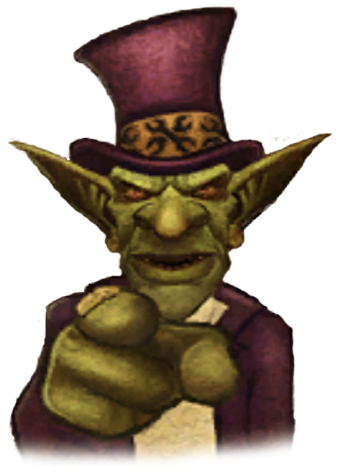
\includegraphics[width=\textwidth,height=5em]{images/le-jeu-video-fiction-ou-realite-2.jpg}

\end{flushright}

\hypertarget{ecritures-dartistes-histoire-duxe9critures-uxe9volutions-et-appropriations-de-luxe9criture}{%
\chapter{\texorpdfstring{Ecritures d'artistes, histoire d'écritures~: \linebreak évolutions et appropriations de l'écriture}{Ecritures d'artistes, histoire d'écritures~: évolutions et appropriations de l'écriture}}\label{ecritures-dartistes-histoire-duxe9critures-uxe9volutions-et-appropriations-de-luxe9criture}}

En 1451, l'homo sapiens d'Europe commençait à imprimer. L'invention de la presse à caractères mobiles permit une double démocratisation, celle de la fabrication de livres et celle de la lecture. L'ancêtre de votre bande-dessinée de Garfield, de votre vocabulaire d'allemand, de vos poèmes de Baudelaire et de vos mangas, c'était un tout premier livre imprimé par Johannes Gutenberg : la grammaire latine de Donatus.

La fabrication d'un livre, même d'un petit livre, nécessite un contenu, donc des images et du texte. Et si c'était à vous de créer un livre~? À l'aide d'outils d'impression anciens et modernes, seriez-vous capables de créer un livre unique~?

\begin{signature}
\emph{Nathalie Fischli}

\end{signature}

\begin{center}\rule{0.5\linewidth}{0.5pt}\end{center}

L'histoire commence avec l'écriture. Cunéiforme, Arial, onciale ou caroline, majuscule ou minuscule, l'écriture évolue et se transforme. Elle s'adapte, elle crée des révolutions. Avec l'apparition de l'imprimerie, les mœurs sont bouleversées. Et presque six cents ans plus tard, à l'heure du numérique, l'écriture manuscrite tend à disparaître.

Ici, vous écrirez sur l'histoire de l'écrit. Pourquoi écrire~? Pourquoi imprimer~? Qui écrit~? Quelles informations méritent-elles de passer à la postérité~? Voici des questions sur lesquelles votre plume (ou votre clavier) pourrait disserter.

\begin{signature}
\emph{Pauline Meylan}

\end{signature}

Travail en binôme recommandé.

\hypertarget{composition-et-ruxe9alisation-dun-ep-clip-viduxe9o-musical}{%
\chapter{Composition et Réalisation d'un EP / clip vidéo musical}\label{composition-et-ruxe9alisation-dun-ep-clip-viduxe9o-musical}}

L'objectif de ce TM est de réaliser un EP à partir de compositions musicales personnelles. Puis vous pourrez réaliser un clip musical à partir de vos compositions.

Dans un premier temps, vous devrez composer la musique et les paroles de votre EP. Ces compositions pourront être faites dans n'importe quel style musical (chanson française, rap, pop, classique,\ldots). Vous devrez vous occuper de l'instrumentation et de l'enregistrement de votre composition en utilisant les logiciels audios (logic pro X, Ableton, Garageband, Pro Tools) pour en réaliser un mix et un Mastering. Vous pourrez vous entourer d'autres musiciens si vous le jugez nécessaire. Enfin, vous devrez présenter un petit clip vidéo pour illustrer une de vos compositions. Vous devrez utiliser un logiciel d'édition vidéo pour la réalisation de celui-ci.

Dans la travail écrit, vous présenterez vos compositions ainsi que les différentes techniques d'édition musicales et vidéo que vous aurez acquises durant tout le processus.

\begin{signature}
\emph{François Voeffray}

\end{signature}

\hypertarget{organisation-dun-concert-public}{%
\chapter{Organisation d'un concert public}\label{organisation-dun-concert-public}}

Le but de ce TM est l'organisation d'un concert public d'environ 45 minutes. L'élève doit s'occuper des lumières, de la sonorisation, de la logistique et de la planification de l'évènement. Il peut s'entourer d'autres musiciens pour son audition. Le style de musique pourra être aussi bien classique que jazz, pop, rock\ldots{}

La partie écrite du TM comportera :

\begin{itemize}
\tightlist
\item
  Une justification du choix du répertoire.
\item
  Les choix et les difficultés inhérents à l'organisation et à la logistique du concert.
\item
  Sa gestion des aspects techniques de la régie
\item
  Les difficultés d'Aufführungspraxis (interprétation) suscitées par les œuvres.
\item
  Un ``livret'' destiné aux spectateurs présentant succinctement chacune des pièces ainsi que les musiciens du concert.
\item
  Un feedback du concert.
\end{itemize}

\begin{signature}
\emph{François Voeffray}

\end{signature}

\hypertarget{pour-prendre-des-notes}{%
\chapter*{Pour prendre des notes}\label{pour-prendre-des-notes}}
\addcontentsline{toc}{chapter}{Pour prendre des notes}

\clearpage

\hypertarget{pour-prendre-plus-de-notes}{%
\subsection*{\ldots{} pour prendre plus de notes}\label{pour-prendre-plus-de-notes}}
\addcontentsline{toc}{subsection}{\ldots{} pour prendre plus de notes}

\end{document}
